% Options for packages loaded elsewhere
\PassOptionsToPackage{unicode}{hyperref}
\PassOptionsToPackage{hyphens}{url}
%
\documentclass[
  man,floatsintext]{apa7}
\usepackage{amsmath,amssymb}
\usepackage{iftex}
\ifPDFTeX
  \usepackage[T1]{fontenc}
  \usepackage[utf8]{inputenc}
  \usepackage{textcomp} % provide euro and other symbols
\else % if luatex or xetex
  \usepackage{unicode-math} % this also loads fontspec
  \defaultfontfeatures{Scale=MatchLowercase}
  \defaultfontfeatures[\rmfamily]{Ligatures=TeX,Scale=1}
\fi
\usepackage{lmodern}
\ifPDFTeX\else
  % xetex/luatex font selection
\fi
% Use upquote if available, for straight quotes in verbatim environments
\IfFileExists{upquote.sty}{\usepackage{upquote}}{}
\IfFileExists{microtype.sty}{% use microtype if available
  \usepackage[]{microtype}
  \UseMicrotypeSet[protrusion]{basicmath} % disable protrusion for tt fonts
}{}
\makeatletter
\@ifundefined{KOMAClassName}{% if non-KOMA class
  \IfFileExists{parskip.sty}{%
    \usepackage{parskip}
  }{% else
    \setlength{\parindent}{0pt}
    \setlength{\parskip}{6pt plus 2pt minus 1pt}}
}{% if KOMA class
  \KOMAoptions{parskip=half}}
\makeatother
\usepackage{xcolor}
\usepackage{graphicx}
\makeatletter
\def\maxwidth{\ifdim\Gin@nat@width>\linewidth\linewidth\else\Gin@nat@width\fi}
\def\maxheight{\ifdim\Gin@nat@height>\textheight\textheight\else\Gin@nat@height\fi}
\makeatother
% Scale images if necessary, so that they will not overflow the page
% margins by default, and it is still possible to overwrite the defaults
% using explicit options in \includegraphics[width, height, ...]{}
\setkeys{Gin}{width=\maxwidth,height=\maxheight,keepaspectratio}
% Set default figure placement to htbp
\makeatletter
\def\fps@figure{htbp}
\makeatother
\setlength{\emergencystretch}{3em} % prevent overfull lines
\providecommand{\tightlist}{%
  \setlength{\itemsep}{0pt}\setlength{\parskip}{0pt}}
\setcounter{secnumdepth}{-\maxdimen} % remove section numbering
% Make \paragraph and \subparagraph free-standing
\ifx\paragraph\undefined\else
  \let\oldparagraph\paragraph
  \renewcommand{\paragraph}[1]{\oldparagraph{#1}\mbox{}}
\fi
\ifx\subparagraph\undefined\else
  \let\oldsubparagraph\subparagraph
  \renewcommand{\subparagraph}[1]{\oldsubparagraph{#1}\mbox{}}
\fi
% definitions for citeproc citations
\NewDocumentCommand\citeproctext{}{}
\NewDocumentCommand\citeproc{mm}{%
  \begingroup\def\citeproctext{#2}\cite{#1}\endgroup}
\makeatletter
 % allow citations to break across lines
 \let\@cite@ofmt\@firstofone
 % avoid brackets around text for \cite:
 \def\@biblabel#1{}
 \def\@cite#1#2{{#1\if@tempswa , #2\fi}}
\makeatother
\newlength{\cslhangindent}
\setlength{\cslhangindent}{1.5em}
\newlength{\csllabelwidth}
\setlength{\csllabelwidth}{3em}
\newenvironment{CSLReferences}[2] % #1 hanging-indent, #2 entry-spacing
 {\begin{list}{}{%
  \setlength{\itemindent}{0pt}
  \setlength{\leftmargin}{0pt}
  \setlength{\parsep}{0pt}
  % turn on hanging indent if param 1 is 1
  \ifodd #1
   \setlength{\leftmargin}{\cslhangindent}
   \setlength{\itemindent}{-1\cslhangindent}
  \fi
  % set entry spacing
  \setlength{\itemsep}{#2\baselineskip}}}
 {\end{list}}
\usepackage{calc}
\newcommand{\CSLBlock}[1]{\hfill\break\parbox[t]{\linewidth}{\strut\ignorespaces#1\strut}}
\newcommand{\CSLLeftMargin}[1]{\parbox[t]{\csllabelwidth}{\strut#1\strut}}
\newcommand{\CSLRightInline}[1]{\parbox[t]{\linewidth - \csllabelwidth}{\strut#1\strut}}
\newcommand{\CSLIndent}[1]{\hspace{\cslhangindent}#1}
\ifLuaTeX
\usepackage[bidi=basic]{babel}
\else
\usepackage[bidi=default]{babel}
\fi
\babelprovide[main,import]{english}
% get rid of language-specific shorthands (see #6817):
\let\LanguageShortHands\languageshorthands
\def\languageshorthands#1{}
% Manuscript styling
\usepackage{upgreek}
\captionsetup{font=singlespacing,justification=justified}

% Table formatting
\usepackage{longtable}
\usepackage{lscape}
% \usepackage[counterclockwise]{rotating}   % Landscape page setup for large tables
\usepackage{multirow}		% Table styling
\usepackage{tabularx}		% Control Column width
\usepackage[flushleft]{threeparttable}	% Allows for three part tables with a specified notes section
\usepackage{threeparttablex}            % Lets threeparttable work with longtable

% Create new environments so endfloat can handle them
% \newenvironment{ltable}
%   {\begin{landscape}\centering\begin{threeparttable}}
%   {\end{threeparttable}\end{landscape}}
\newenvironment{lltable}{\begin{landscape}\centering\begin{ThreePartTable}}{\end{ThreePartTable}\end{landscape}}

% Enables adjusting longtable caption width to table width
% Solution found at http://golatex.de/longtable-mit-caption-so-breit-wie-die-tabelle-t15767.html
\makeatletter
\newcommand\LastLTentrywidth{1em}
\newlength\longtablewidth
\setlength{\longtablewidth}{1in}
\newcommand{\getlongtablewidth}{\begingroup \ifcsname LT@\roman{LT@tables}\endcsname \global\longtablewidth=0pt \renewcommand{\LT@entry}[2]{\global\advance\longtablewidth by ##2\relax\gdef\LastLTentrywidth{##2}}\@nameuse{LT@\roman{LT@tables}} \fi \endgroup}

% \setlength{\parindent}{0.5in}
% \setlength{\parskip}{0pt plus 0pt minus 0pt}

% Overwrite redefinition of paragraph and subparagraph by the default LaTeX template
% See https://github.com/crsh/papaja/issues/292
\makeatletter
\renewcommand{\paragraph}{\@startsection{paragraph}{4}{\parindent}%
  {0\baselineskip \@plus 0.2ex \@minus 0.2ex}%
  {-1em}%
  {\normalfont\normalsize\bfseries\itshape\typesectitle}}

\renewcommand{\subparagraph}[1]{\@startsection{subparagraph}{5}{1em}%
  {0\baselineskip \@plus 0.2ex \@minus 0.2ex}%
  {-\z@\relax}%
  {\normalfont\normalsize\itshape\hspace{\parindent}{#1}\textit{\addperi}}{\relax}}
\makeatother

\makeatletter
\usepackage{etoolbox}
\patchcmd{\maketitle}
  {\section{\normalfont\normalsize\abstractname}}
  {\section*{\normalfont\normalsize\abstractname}}
  {}{\typeout{Failed to patch abstract.}}
\patchcmd{\maketitle}
  {\section{\protect\normalfont{\@title}}}
  {\section*{\protect\normalfont{\@title}}}
  {}{\typeout{Failed to patch title.}}
\makeatother

\usepackage{xpatch}
\makeatletter
\xapptocmd\appendix
  {\xapptocmd\section
    {\addcontentsline{toc}{section}{\appendixname\ifoneappendix\else~\theappendix\fi\\: #1}}
    {}{\InnerPatchFailed}%
  }
{}{\PatchFailed}
\keywords{cross-cultural psychology, social cognition, gaze following, individual differences, reliability\newline\indent Word count: XXX}
\usepackage{lineno}

\linenumbers
\usepackage{csquotes}
\usepackage{amsmath}
\usepackage{amssymb}
\usepackage{unicode-math}
\usepackage{setspace}
\usepackage{libertine}
\captionsetup[figure]{font={stretch=1}}
\makeatletter
\renewcommand{\paragraph}{\@startsection{paragraph}{4}{\parindent}%
  {0\baselineskip \@plus 0.2ex \@minus 0.2ex}%
  {-1em}%
  {\normalfont\normalsize\bfseries\typesectitle}}

\renewcommand{\subparagraph}[1]{\@startsection{subparagraph}{5}{1em}%
  {0\baselineskip \@plus 0.2ex \@minus 0.2ex}%
  {-\z@\relax}%
  {\normalfont\normalsize\bfseries\itshape\hspace{\parindent}{#1}\textit{\addperi}}{\relax}}
\makeatother

\ifLuaTeX
  \usepackage{selnolig}  % disable illegal ligatures
\fi
\usepackage{bookmark}
\IfFileExists{xurl.sty}{\usepackage{xurl}}{} % add URL line breaks if available
\urlstyle{same}
\hypersetup{
  pdftitle={Measuring variation in gaze following across communities, ages, and individuals --- a showcase of the TANGO-CC},
  pdfauthor={Julia Christin Prein (ORCID: 0000-0002-3154-6167)1,2, Florian M. Bednarski (ORCID: 0000-0003-4384-4791)3, Ardain Dzabatou4, Michael C. Frank (ORCID: 0000-0002-7551-4378)5, Annette M. E. Henderson (ORCID: 0000-0003-4384-4791)3, Josefine Kalbitz2, Patricia Kanngiesser (ORCID:0000-0003-1068-3725)6, Dilara Keşşafoğlu (ORCID: 0000-0002-7356-0733)7, Bahar Köymen (ORCID: 0000-0001-5126-8240)8, Maira V. Manrique-Hernandez2, Shirley Magazi (ORCID: 0009-0006-0479-9800)9, Lizbeth Mújica-Manrique2, Julia Ohlendorf2, Damilola Olaoba2, Wesley R. Pieters (ORCID:0000-0002-6152-249X)9, Sarah Pope-Caldwell2,10, Umay Sen (ORCID: 0000-0001-9488-0851)11, Katie Slocombe (ORCID: 0000-0002-7310-1887)12, Robert Z. Sparks (ORCID: 0000-0001-7545-0522)5, Roman Stengelin (ORCID: 0000-0003-2212-4613)2,9, Jahnavi Sunderarajan2, Kirsten Sutherland2, Florence Tusiime13, Wilson Vieira (ORCID: 0009-0001-9400-6328)2, Zhen Zhang (ORCID: 0000-0001-9300-0920)14, Yufei Zong (ORCID: 0009-0000-5012-0244)14,15, Daniel B. M. Haun (ORCID: 0000-0002-3262-645X)2,+, \& Manuel Bohn (ORCID: 0000-0001-6006-1348)1,2,+},
  pdflang={en-EN},
  pdfkeywords={cross-cultural psychology, social cognition, gaze following, individual differences, reliability},
  hidelinks,
  pdfcreator={LaTeX via pandoc}}

\title{Measuring variation in gaze following across communities, ages, and individuals --- a showcase of the TANGO-CC}
\author{Julia Christin Prein (ORCID: 0000-0002-3154-6167)\textsuperscript{1,2}, Florian M. Bednarski (ORCID: 0000-0003-4384-4791)\textsuperscript{3}, Ardain Dzabatou\textsuperscript{4}, Michael C. Frank (ORCID: 0000-0002-7551-4378)\textsuperscript{5}, Annette M. E. Henderson (ORCID: 0000-0003-4384-4791)\textsuperscript{3}, Josefine Kalbitz\textsuperscript{2}, Patricia Kanngiesser (ORCID:0000-0003-1068-3725)\textsuperscript{6}, Dilara Keşşafoğlu (ORCID: 0000-0002-7356-0733)\textsuperscript{7}, Bahar Köymen (ORCID: 0000-0001-5126-8240)\textsuperscript{8}, Maira V. Manrique-Hernandez\textsuperscript{2}, Shirley Magazi (ORCID: 0009-0006-0479-9800)\textsuperscript{9}, Lizbeth Mújica-Manrique\textsuperscript{2}, Julia Ohlendorf\textsuperscript{2}, Damilola Olaoba\textsuperscript{2}, Wesley R. Pieters (ORCID:0000-0002-6152-249X)\textsuperscript{9}, Sarah Pope-Caldwell\textsuperscript{2,10}, Umay Sen (ORCID: 0000-0001-9488-0851)\textsuperscript{11}, Katie Slocombe (ORCID: 0000-0002-7310-1887)\textsuperscript{12}, Robert Z. Sparks (ORCID: 0000-0001-7545-0522)\textsuperscript{5}, Roman Stengelin (ORCID: 0000-0003-2212-4613)\textsuperscript{2,9}, Jahnavi Sunderarajan\textsuperscript{2}, Kirsten Sutherland\textsuperscript{2}, Florence Tusiime\textsuperscript{13}, Wilson Vieira (ORCID: 0009-0001-9400-6328)\textsuperscript{2}, Zhen Zhang (ORCID: 0000-0001-9300-0920)\textsuperscript{14}, Yufei Zong (ORCID: 0009-0000-5012-0244)\textsuperscript{14,15}, Daniel B. M. Haun (ORCID: 0000-0002-3262-645X)\textsuperscript{2,+}, \& Manuel Bohn (ORCID: 0000-0001-6006-1348)\textsuperscript{1,2,+}}
\date{}


\shorttitle{measuring gaze following across communities}

\authornote{

The authors made the following contributions. Julia Christin Prein (ORCID: 0000-0002-3154-6167): Conceptualization, Formal Analysis, Methodology, Project administration, Resources, Software, Visualization, Writing - Original Draft Preparation, Writing - Review \& Editing; Florian M. Bednarski (ORCID: 0000-0003-4384-4791): Methodology, Resources, Writing - Review \& Editing; Ardain Dzabatou: Methodology, Resources, Writing - Review \& Editing; Michael C. Frank (ORCID: 0000-0002-7551-4378): Methodology, Resources, Writing - Review \& Editing; Annette M. E. Henderson (ORCID: 0000-0003-4384-4791): Methodology, Resources, Writing - Review \& Editing; Josefine Kalbitz: Methodology, Resources, Writing - Review \& Editing; Patricia Kanngiesser (ORCID:0000-0003-1068-3725): Methodology, Resources, Writing - Review \& Editing; Dilara Keşşafoğlu (ORCID: 0000-0002-7356-0733): Methodology, Resources, Writing - Review \& Editing; Bahar Köymen (ORCID: 0000-0001-5126-8240): Methodology, Resources, Writing - Review \& Editing; Maira V. Manrique-Hernandez: Methodology, Resources, Writing - Review \& Editing; Shirley Magazi (ORCID: 0009-0006-0479-9800): Methodology, Resources, Writing - Review \& Editing; Lizbeth Mújica-Manrique: Methodology, Resources, Writing - Review \& Editing; Julia Ohlendorf: Methodology, Resources, Writing - Review \& Editing; Damilola Olaoba: Methodology, Resources, Writing - Review \& Editing; Wesley R. Pieters (ORCID:0000-0002-6152-249X): Methodology, Resources, Writing - Review \& Editing; Sarah Pope-Caldwell: Methodology, Resources, Writing - Review \& Editing; Umay Sen (ORCID: 0000-0001-9488-0851): Methodology, Resources, Writing - Review \& Editing; Katie Slocombe (ORCID: 0000-0002-7310-1887): Methodology, Resources, Writing - Review \& Editing; Robert Z. Sparks (ORCID: 0000-0001-7545-0522): Methodology, Resources, Writing - Review \& Editing; Roman Stengelin (ORCID: 0000-0003-2212-4613): Conceptualization, Methodology, Resources, Writing - Review \& Editing; Jahnavi Sunderarajan: Methodology, Resources, Writing - Review \& Editing; Kirsten Sutherland: Methodology, Resources, Writing - Review \& Editing; Florence Tusiime: Methodology, Resources, Writing - Review \& Editing; Wilson Vieira (ORCID: 0009-0001-9400-6328): Methodology, Resources, Writing - Review \& Editing; Zhen Zhang (ORCID: 0000-0001-9300-0920): Methodology, Resources, Writing - Review \& Editing; Yufei Zong (ORCID: 0009-0000-5012-0244): Methodology, Resources, Writing - Review \& Editing; Daniel B. M. Haun (ORCID: 0000-0002-3262-645X): Conceptualization, Funding acquisition, Methodology, Writing - Review \& Editing; Manuel Bohn (ORCID: 0000-0001-6006-1348): Conceptualization, Funding acquisition, Methodology, Project administration, Supervision, Writing - Review \& Editing.

Correspondence concerning this article should be addressed to Julia Christin Prein (ORCID: 0000-0002-3154-6167), Universitätsallee 1, 21335 Lüneburg, Germany. E-mail: \href{mailto:julia.prein@leuphana.de}{\nolinkurl{julia.prein@leuphana.de}}

}

\affiliation{\vspace{0.5cm}\textsuperscript{1} Institute of Psychology in Education, Leuphana University Lüneburg, Germany\\\textsuperscript{2} Department of Comparative Cultural Psychology, Max Planck Institute for Evolutionary Anthropology, Germany\\\textsuperscript{3} School of Psychology, University of Auckland, New Zealand\\\textsuperscript{4} Université Marien Ngouabi, Republic of the Congo\\\textsuperscript{5} Department of Psychology, Stanford University, USA\\\textsuperscript{6} School of Psychology, University of Plymouth, UK\\\textsuperscript{7} Department of Psychology, Koç University, Türkiye\\\textsuperscript{8} Division of Psychology, Communication, and Human Neuroscience, University of Manchester, UK\\\textsuperscript{9} Department of Psychology and Social Work, University of Namibia, Namibia\\\textsuperscript{10} Department of Psychology, Georgia State University, USA\\\textsuperscript{11} Department of Psychology, Developmental Psychology, Uppsala University, Sweden\\\textsuperscript{12} Department of Psychology, University of York, UK\\\textsuperscript{13} Budongo Conservation Field Station, Uganda\\\textsuperscript{14} CAS Key Laboratory of Behavioral Science, Institute of Psychology, Chinese Academy of Sciences, China\\\textsuperscript{15} Department of Cognitive Sciences, University of California Irvine, USA\\\textsuperscript{+} joint last author}

\abstract{%
Cross-cultural studies are crucial for investigating the cultural variability and universality of cognitive developmental processes. However, cross-cultural assessment tools in cognition across languages and communities are limited. This paper describes a gaze following task designed to measure basic social cognition across individuals, ages, and communities (TANGO-CC). The task was developed and psychometrically assessed in one cultural setting and, with input of local collaborators, adapted for cross-cultural data collection. Minimal language demands and the web-app implementation allow fast and easy contextual adaptations to each community. The TANGO-CC captures individual- and community-level variation and shows good internal consistency in a data set from 2.5- to 11-year-old children from 17 diverse communities. Within-community variation outweighed between-community variation. We provide an open-source website for researchers to customize and use the task (\url{https://ccp-odc.eva.mpg.de/tango-cc}). The TANGO-CC can be used to assess basic social cognition in diverse communities and provides a roadmap for researching community-level and individual-level differences across cultures.
}



\begin{document}
\maketitle

\section{Introduction}\label{introduction}

For decades, researchers have advocated for more diverse samples in psychological research and cautioned against relying solely on convenience samples from the Global North (Arnett, 2008; Henrich et al., 2010; Lillard, 1998).
Despite numerous calls for change, the samples reported in major psychology journals still lack diversity (Apicella et al., 2020; Gutchess \& Rajaram, 2023; Thalmayer et al., 2021).
This hinders progress in theory building and testing: we cannot draw inferences about universal and variable aspects of the human cognitive system from data collected exclusively in one single community (Krys et al., 2024).
While this sampling bias is often discussed within adult psychology, it is equally relevant to developmental psychology (Nielsen et al., 2017).
Early experiences shape the way children think about and interact with the world and an ontogenetic perspective is needed to explore the foundational aspects of human behavioral diversity (Amir \& McAuliffe, 2020; Broesch et al., 2023; Liebal \& Haun, 2018; Torréns et al., 2023).

There are numerous challenges with collecting cross-cultural, developmental data (Amir \& McAuliffe, 2020; Broesch et al., 2023).
Cross-cultural studies need reliable and valid measures to capture variation between communities and/or individuals systematically.
Even though this applies to all areas of cognitive development, we focus on social cognition in this paper.

Social cognition refers to how an individual processes information in social situations which allows them to understand and predict others' behavior (Adolphs, 1999; Decety, 2020; Frith \& Frith, 2007; Zeigler-Hill et al., 2015).
If, in theory, stimuli used in social cognition tasks should relate to people's everyday experiences, then tasks themselves should be tuned to the features of specific communities.
Indeed, task performance can be diminished when stimuli do not reflect the characteristics of the participants' communities (Peña, 2007).
For example, Elfenbein and Ambady (2002) found better emotion recognition for members of the same national, ethnic, or regional group.
Selcuk et al. (2023) concluded that children often attribute mental states more accurately and more frequently to individuals from the same community.

From a psychometric perspective, the situation looks dire. Studies on social cognition with US-American and European samples rarely report psychometric information (for a review, see Beaudoin et al., 2020), and the picture further deteriorates when we look at cross-cultural social cognition tasks (Bourdage et al., 2023; Hajdúk et al., 2020; Waschl \& Chen, 2022).
Thus, it is already challenging to find reliable and valid tasks that have measurement sensitivity to detect individual differences within one community, let alone tasks that do so across different communities.
In this paper, we describe the construction and psychometric evaluation of a cross-cultural measure of basic social cognition (gaze following) in children as a concrete example of how to address this problem.

The approaches that researchers can take to collect cross-cultural data lie on a continuum: the decision for a specific method partly depends on whether researchers aim to increase the \emph{depth} (culture specificity) or \emph{breadth} (standardization across multiple communities) of their work (Amir \& McAuliffe, 2020).
At one extreme, researchers translate the psychological construct into a separate design or task for each community (termed ``assembly''; He and Vijver (2012), Waschl and Chen (2022)).
While this approach allows greater flexibility and sensitivity to cultural differences, it might not be feasible to study a multitude of communities as it becomes too demanding and time-consuming.
Furthermore, the results are limited to each community and absolute task scores might not be comparable across communities.
A study following this approach is Wefers et al. (2023) who investigated how cultural variations in parenting styles modulated infants' responses to disruptions in social interactions.
While studies in the Global North often apply the Still-Face Paradigm to assess infants' reactions to unresponsive partners, Wefers et al. (2023) reasoned that this paradigm might not capture infants' everyday interaction routines in communities with proximal (i.e., emphasis on body stimulation) parenting styles.
By developing the novel No-Touch Paradigm, they found that indeed infants' responses to unresponsive partners were modulated by the cultural context in which they grew up: Kichwa infants from rural Ecuador showed stronger reactions to unresponsive partners in the No-Touch Paradigm compared to the Still-Face Paradigm, while reactions of urban German infants differed less in both paradigms.

At the other extreme, researchers use the same standardized procedure across diverse communities, potentially providing a simple translation or modification of stimuli to ensure they are culturally appropriate (termed ``adoption'' and ``adaptation'', respectively; He and Vijver (2012), Waschl and Chen (2022)).
This approach is less sensitive to each community's unique characteristics but renders quantitative comparisons of data more feasible.
An example following this approach is the Multilingual Assessment Instrument for Narratives (MAIN; Gagarina et al. (2012)), which assesses narrative abilities in mono- and multilingual children.
Extensive piloting and adaptation of MAIN materials ensured that the instrument is culturally appropriate, robust, and suitable for cross-linguistic comparisons (Gagarina et al., 2012), and new and revised language versions are continuously added to the MAIN database (Gagarina \& Lindgren, 2020).

The present paper aims to describe the development and psychometric properties of a social cognition task that can be adapted to diverse communities.
On the continuum described above, our task lies more toward standardized approaches but allows for some customization of the stimuli to each local community.
The task focuses on one of the most fundamental social-cognitive abilities: gaze following, that is, the ability to identify the attentional focus of another agent.
Gaze following develops early in infancy (Del Bianco et al., 2019; Tang et al., 2024) and contributes to social learning, communication, and collaboration (Bohn \& Köymen, 2018; Hernik \& Broesch, 2019; Shepherd, 2010; Tomasello et al., 2007).
Identifying the attentional focus of a conversational partner facilitates language development (Brooks \& Meltzoff, 2015; Carpenter et al., 1998; Mundy et al., 2007), as children might use gaze to identify the referent of a new word (Brooks \& Meltzoff, 2005).

One of the main open questions is the impact of social-environmental and cultural factors on gaze following (Astor \& Gredebäck, 2022), but studies on variation in gaze following across communities are rare.
Recently, Brooks et al. (2020) found that Deaf infants show increased gaze following compared to hearing infants, underlining the importance of visual-communicative signals for Deaf children.
Callaghan et al. (2011) investigated gaze following behind barriers in 12- and 17-month-olds from rural Canada (n = 35), Peru (n = 38), and India (n = 65).
In their setup, an agent looked at a toy behind (experimental condition) or a sticker in front of (control condition) a barrier, and children's crawling toward the barrier to follow the agent's gaze was assessed.
While the absolute crawling rates differed across communities, children in all three communities crawled more often to gain visual access when the agent looked at an object behind the barrier than in front of it.
Hernik and Broesch (2019) studied 22 infants between 5 to 7 months of age from Vanuatu and used an eye-tracking procedure displaying a local actor looking at one of two objects.
Even though face-to-face interactions are less common in parent-child interactions in Vanuatu than in Western communities, the result patterns of gaze following in Ni-Vanuatu infants resembled those of their Western counterparts: infants from Vanuatu followed the agent's gaze to the target object only when preceded by infant-directed, and not adult-directed, speech.
Astor et al. (2022) analyzed the effects of maternal postpartum depression on gaze following in 9-month-olds from Bhutan and Sweden. While infants showed similar gaze following rates in both countries, maternal postpartum depression was associated with reduced gaze following only in the Swedish sample.
Beyond gaze following, some studies conducted in the Global South have investigated opportunities for mutual eye gaze and factors influencing joint attention (see Akhtar \& Gernsbacher, 2008).
For example, Kaluli infants in Papua New Guinea are often carried facing away from their mothers so infants and caregivers share mutual gaze less frequently (Ochs \& Schieffelin, 1984). Childers et al. (2007) studied Ngas-speaking infants in Nigeria and found no effect of the caregivers' carrying style (usually on the back) on children's joint attention tendencies.

While these studies point towards potential cross-cultural stability of gaze following, the lack of psychometrically evaluated tasks and the small number of communities studied limit the generalizability of these findings and -- more importantly -- does not allow for studying individual-differences.
A more comprehensive cross-cultural study on gaze following was recently conducted by Bohn, Prein, et al. (2024). The researchers tested the universality of gaze following by studying 17 different communities on five continents and found evidence for a similar processing mechanism across communities.

The task presented in this manuscript was developed for the study by Bohn, Prein, et al. (2024) and is based on a previously established gaze-following task called `TANGO' (Task for Assessing iNdividual differences in Gaze understanding - Open) by Prein, Kalinke, et al. (2024).
The TANGO measures how precisely participants locate an agent's attentional focus.
It reliably measured individual differences in a German child sample and an English-speaking remote adult sample (Prein, Kalinke, et al., 2024).
However, we cannot claim the task's generalizability and reliability based on a mono-cultural sample.
This paper showcases the TANGO-CC (TANGO - Cross-Cultural), a standardized gaze following task that has been adapted to 13 languages and even more communities, and evaluates its psychometric properties by leveraging a large and diverse data set of 2.5- to 11-year-olds from 17 diverse communities (Bohn, Prein, et al., 2024).
We describe the task's development and provide a tutorial for the open-source website (\url{https://ccp-odc.eva.mpg.de/tango-cc/}).

\section{Task development}\label{task-development}

\subsection{Approach}\label{approach}

The TANGO-CC was implemented in Leipzig, Germany, and thoroughly assessed in terms of reliability and validity (Prein, Kalinke, et al., 2024).
During this process, the cross-cultural adaptation of the task was prepared by a team of cross-cultural psychologists and cognitive scientists.
In this paper, we assess the TANGO-CC's measurement quality (i.e., variability and reliability) across 17 diverse communities by analyzing the data set from Bohn, Prein, et al. (2024).
In the following, we describe the different steps in detail.

The TANGO-CC is a screen-based, interactive picture book with cartoon-like line drawings (see Figure \ref{fig:fig1}). Previous gaze studies have successfully implemented tasks with (schematic) line drawings for both children and adults (e.g., Anderson \& Doherty, 1997; Doherty et al., 2009; Doherty \& Anderson, 1999; Kingstone et al., 2000; Lee et al., 1998).
The TANGO-CC measures the imprecision with which participants locate a balloon by following an agent's gaze.
Participants click or touch the location on the screen where they believe the balloon to be.
Precision is measured as the distance between the participant's click on the screen and the balloon's real position.

During the task development, we decided to implement the task's main functionality independently of the task's appearance.
We programmed a function that calculates the x and y coordinates of where the agent's pupil and iris should move to follow the balloon, given the eyes' and balloon's original positions and measures.
As the measures of the eyes and balloon are read out dynamically from the image on screen, stimuli can be easily adapted and exchanged (i.e., no coordination values for animation are hard-coded into the task's source code).
After having programmed this ``backbone'' functionality of the task (i.e., animate the eyes so that they follow the balloon), we added the task's audio instructions and superficial appearance (e.g., background scene, hedge, agent faces).

This basic version of the TANGO was psychometrically evaluated in a German child sample and an English-speaking remote adult sample and was found to be highly reliable and valid (Prein, Kalinke, et al., 2024).
While children became more precise in locating the agent's attentional focus with age, individuals differed across all age groups and showed no floor- or ceiling effects.
In the Leipzig sample, performance in the TANGO was weakly related to factors of children's daily social environment and could predict children's receptive vocabulary 6 months later.
In a computational cognitive model, Prein, Maurits, et al. (2024) described gaze following as a form of social vector following and empirically found that performance in the TANGO was related to children's non-social vector following and visual perspective-taking abilities.
These connections to related constructs indicate the task's convergent validity in the German child sample.

To adapt the task for cross-cultural data collection, we generated a set of human cartoon faces and background scenes with input from local researchers and research assistants.
The stimulus pool was adjusted and expanded until the researchers and research assistants from each target community judged the selected stimuli to be representative of the local population and typical accommodation (see Figure \ref{fig:fig2}).
Audio instructions were translated from English or German into the corresponding local language(s).
By back-translating these instructions, we ensured the original meaning did not change.
Sometimes, specific words were slightly modified in the target language (e.g., ``bush'' instead of ``hedge'') to ensure that all participants understood the instructions well.
Based on these adaptations, the TANGO-CC could be applied in 17 communities and 13 different languages (Bohn, Prein, et al., 2024). In the following, we describe how researchers can use and customize the TANGO-CC in more detail.

\subsection{Features of the TANGO-CC}\label{features-of-the-tango-cc}

\subsubsection{Trials}\label{trials}



\begin{figure}

{\centering 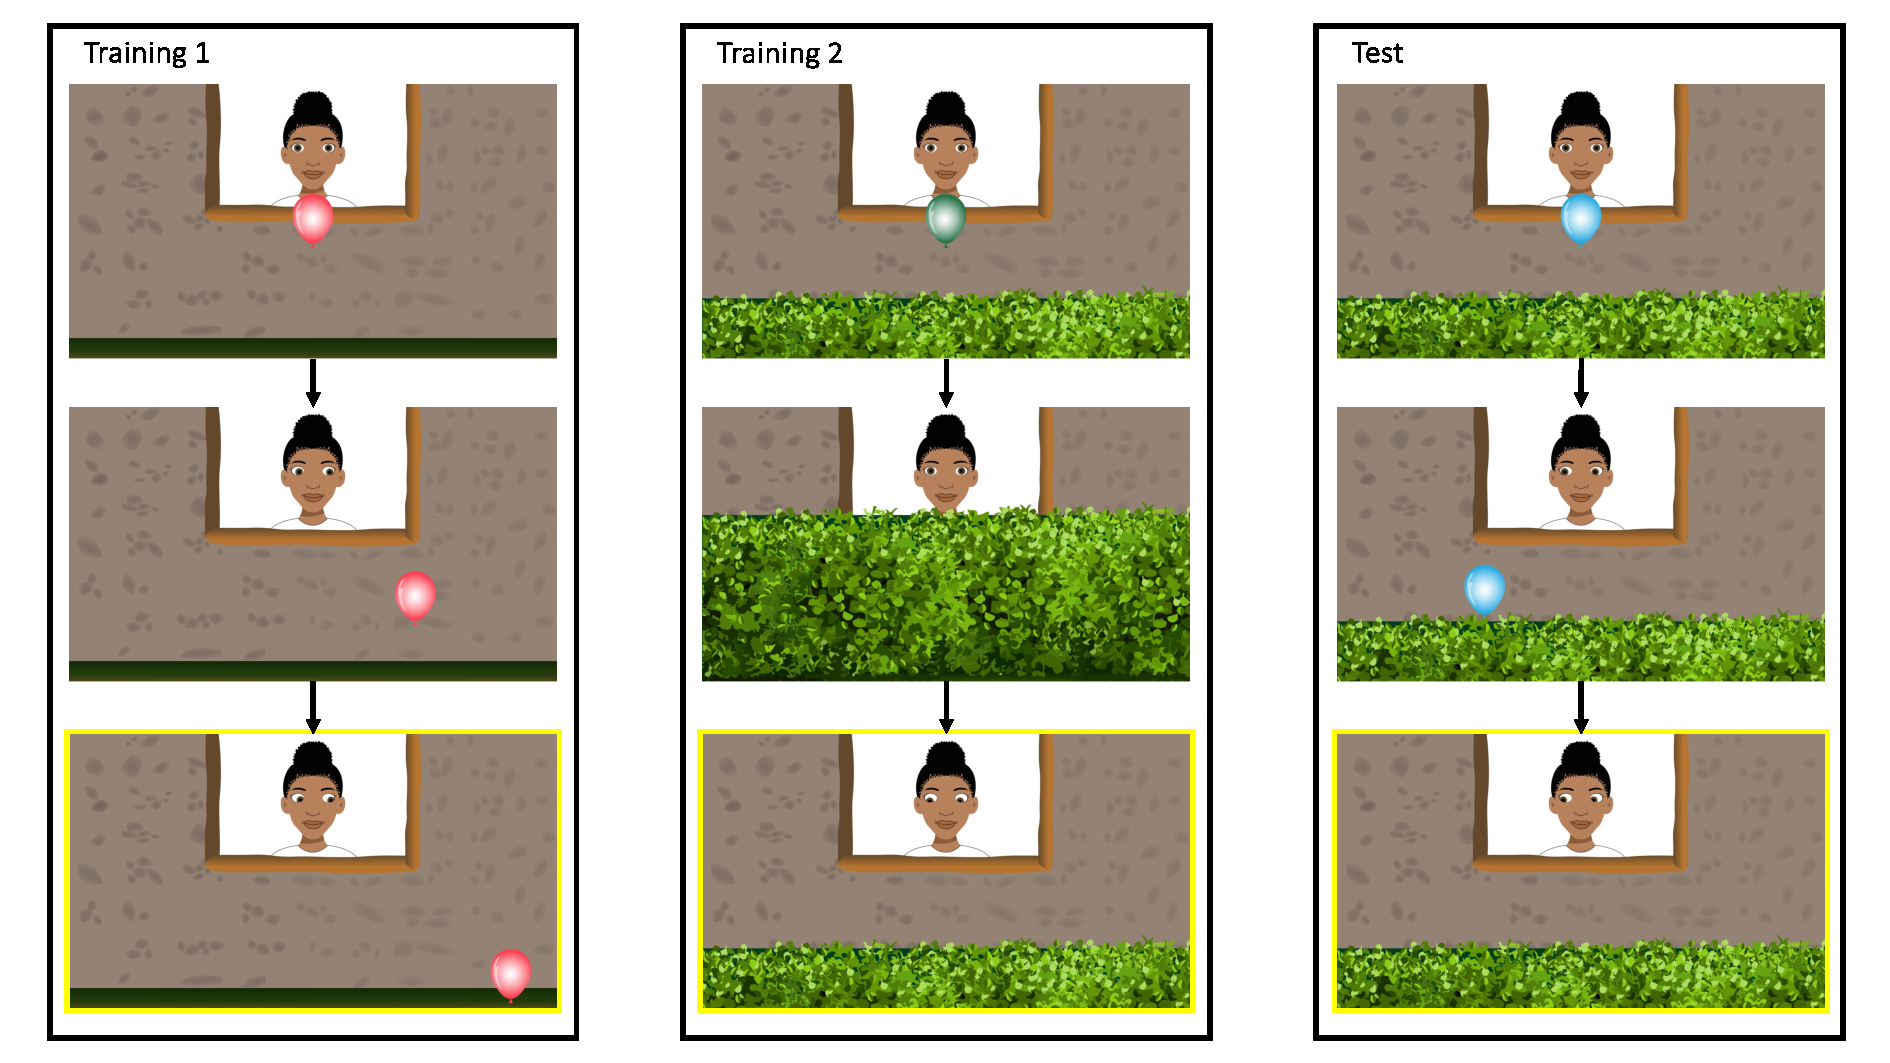
\includegraphics[width=1\linewidth]{../figures/tango-cc-procedure} 

}

\caption{\textbf{Screenshots of the trials.} In training 1, an agent looks at a balloon that falls to the ground, and participants have to respond by clicking/touching the balloon. In training 2, the balloon falls behind the hedge while its flight is still visible. Participants respond by clicking the hedge where they think the balloon is. In test trials, the balloon's movement and final position are covered by a hedge, and participants respond by clicking the hedge. In the task, all movements are smoothly animated (no still pictures). Yellow frames indicate the time point when participants respond (only illustrative, not shown during the task).}\label{fig:fig1}
\end{figure}

The task consists of three different trial types: training 1, training 2, and test trials (see Figure \ref{fig:fig1}).
In every trial, participants see an agent (boy or girl) looking out of a house with a balloon (red, blue, green, or yellow) in front of them.
The balloon falls down to the ground. The eyes of the agent follow the movement of the balloon in a way that the balloon center and the pupil center always align.
Depending on the trial type, participants' visual access to the balloon's position varies.
This experimental design builds on existing gaze following paradigms that have used barriers or obstacles (e.g., Butler et al., 2000; Dunphy-Lelii \& Wellman, 2004; Franco \& Gagliano, 2001; Moll \& Tomasello, 2004).
In training 1, participants see the full trajectory of the balloon and directly have to click the balloon itself.
In training 2, participants see most of the balloon's movement, but a hedge covers the final location.
In test trials, a hedge grows at the beginning of the trial and participants see neither the movement nor the final position of the balloon.

The first trial of each type contains an audio description of the presented events (see Supplements).
Notably, the instructions explicitly state that the agent is looking at the balloon.
This ensures all participants understand the purpose of the task, and minimizes learning effects (increasing comparability between earlier and later trials; avoiding that participants notice the gaze cue only after e.g.~half of the trials).
The TANGO-CC measures \emph{how precisely} participants use the gaze cue, rather than \emph{if} they notice it in the first place.

The outcome variable is the distance between the participant's click and the balloon's center.
Trials can be completed quickly and efficiently so that children can complete 15 trials within 10 minutes, and few children fail to complete the task.
By using self-explanatory animations, language demands are kept to a minimum.
The task uses simple audio instructions, which makes the task accessible to children from different age groups, and no reading skills are required.
There is no feedback during the task to prevent learning effects across trials.

\subsubsection{Randomization}\label{randomization}

The order of the agents, balloon colors (red, yellow, green, blue), and balloon positions are each randomized independently.
For the balloon positions, the entire width of the screen (1920 in ``SVG units'') is divided into ten bins.
Exact coordinates (value between 0 for the far left and 1920 for the far right) within each bin are then randomly generated.
The number of repetitions for each agent, balloon color, and balloon bin is calculated based on the total number of trials and the number of unique agents, balloon colors, and bins, respectively.
All agents, balloon colors, and bins appear equally often and are not repeated in more than two consecutive trials.
If the total number of trials is not divisible by the number of unique elements, some elements (i.e., some agents, balloon colors, bins) are randomly repeated to make up for the remainder.

\subsubsection{Cross-cultural customization}\label{cross-cultural-customization}

When researchers visit the TANGO-CC's website
(\url{https://ccp-odc.eva.mpg.de/tango-cc/}), they can select the language for audio instructions which are currently available for 13 different languages and five more dialects (see Table 1).
To add a new language, researchers have two options:
(1) for using their own audio instructions in the offline version of the task, researchers can download the task, exchange the audio instructions in the dist folder (in the folder sounds \textgreater{} custom) and select ``Custom'' in the language drop-down menu.
For detailed instructions, see the TANGO-CC's manual (\url{https://ccp-odc.eva.mpg.de/tango-cc/manual.html}).
(2) For adding a new language in the online version of the task, researchers can contact the first author of this paper. Please note that this option requires new audio recordings by the interested researchers, which will then be openly available for all users of the task.
All written instructions in the task are solely for the research assistant to help them guide participants through the task; these instructions are solely available in English.
The task can either be started with the default settings or further customized by adapting the number of trials, agents, and background scenes.
The default settings use the version applied in Bohn, Prein, et al. (2024) based on the selected language (see Supplements).

If researchers choose to customize the task (see Figure \ref{fig:fig2}), they can adjust the number of trials for each trial type, but not their sequence.
Specifically, trial types build on each other and participants need to complete each trial type (without skipping any) to understand the structure of the task.
The minimum number of trials per type is 1; the maximum is 100.
Furthermore, researchers can customize backgrounds by selecting one of four different backgrounds.
Finally, researchers can choose from 50 diverse cartoon-like human faces (50\% female, 50\% male) and freely select how many different faces to include (min 1, max 50).
Once all the settings are selected, the customized task is compiled.
To save the selected settings, researchers can bookmark the URL to easily access the customized task.

In the last step, researchers can enter an alphanumeric participant identifier (1 - 8 characters) and enable a webcam recording of the participant, if needed.
A webcam recording might prove especially helpful for unsupervised online data collection to ensure that the participant is alone during the task and no help is provided.
The participant identifier and webcam choice have to be provided every time the task is run.

The source code of the task is openly available on GitHub (\url{https://github.com/ccp-eva/tango-cc}).
By directly editing the \texttt{HTML} and \texttt{JavaScript} code, researchers can further modify the task as needed.
To ensure the accessibility of the TANGO--CC long-term, we have additionally stored the source code on Zenodo (\url{https://zenodo.org/doi/10.5281/zenodo.13643836}).

We created a public OSF page (\url{https://doi.org/10.17605/OSF.IO/P2EGU}) on which we plan to collect data sets that used the TANGO-CC.
Researchers who have collected data using the TANGO-CC can share their data with the community by contacting the first author of this paper or visiting the OSF repository.

\begin{table}[tbp]

\begin{center}
\begin{threeparttable}

\caption{\label{tab:langtab}Current language options available for the audio instructions in the TANGO-CC}

\begin{tabular}{lll}
\toprule
Languages & \multicolumn{1}{c}{Language family} & \multicolumn{1}{c}{Speaker's country of origin}\\
\midrule
Bemba & Bantu & Zambia\\
Chinese & Sino-Tibetan & China\\
English & Indo-European & USA / UK / India / Nigeria / New Zealand\\
German & Indo-European & Germany\\
(≠Akhoe) Hai||om & Khoe-Kwadi & Namibia\\
Khwedam & Khoe-Kwadi & Namibia\\
Lingala & Bantu & Rep. Congo\\
Marathi & Indo-European & India\\
Shona * & Bantu & Zimbabwe\\
Spanish & Indo-European & Argentina (Rioplatense Spanish) / Mexico (Mexiquense Spanish)\\
Kiswahili & Bantu & Uganda\\
Turkish & Turkic & Türkiye\\
Yaka & Bantu & Rep. Congo\\
\bottomrule
\addlinespace
\end{tabular}

\begin{tablenotes}[para]
\normalsize{\textit{Note.} In cases where more than one speaker's country of origin is listed, the audio instructions were recorded multiple times by different speakers. For example, the English instructions are available in five different versions. * Please note that audio instructions are available in Shona but no data of this version is included in the present data set.}
\end{tablenotes}

\end{threeparttable}
\end{center}

\end{table}



\begin{figure}

{\centering 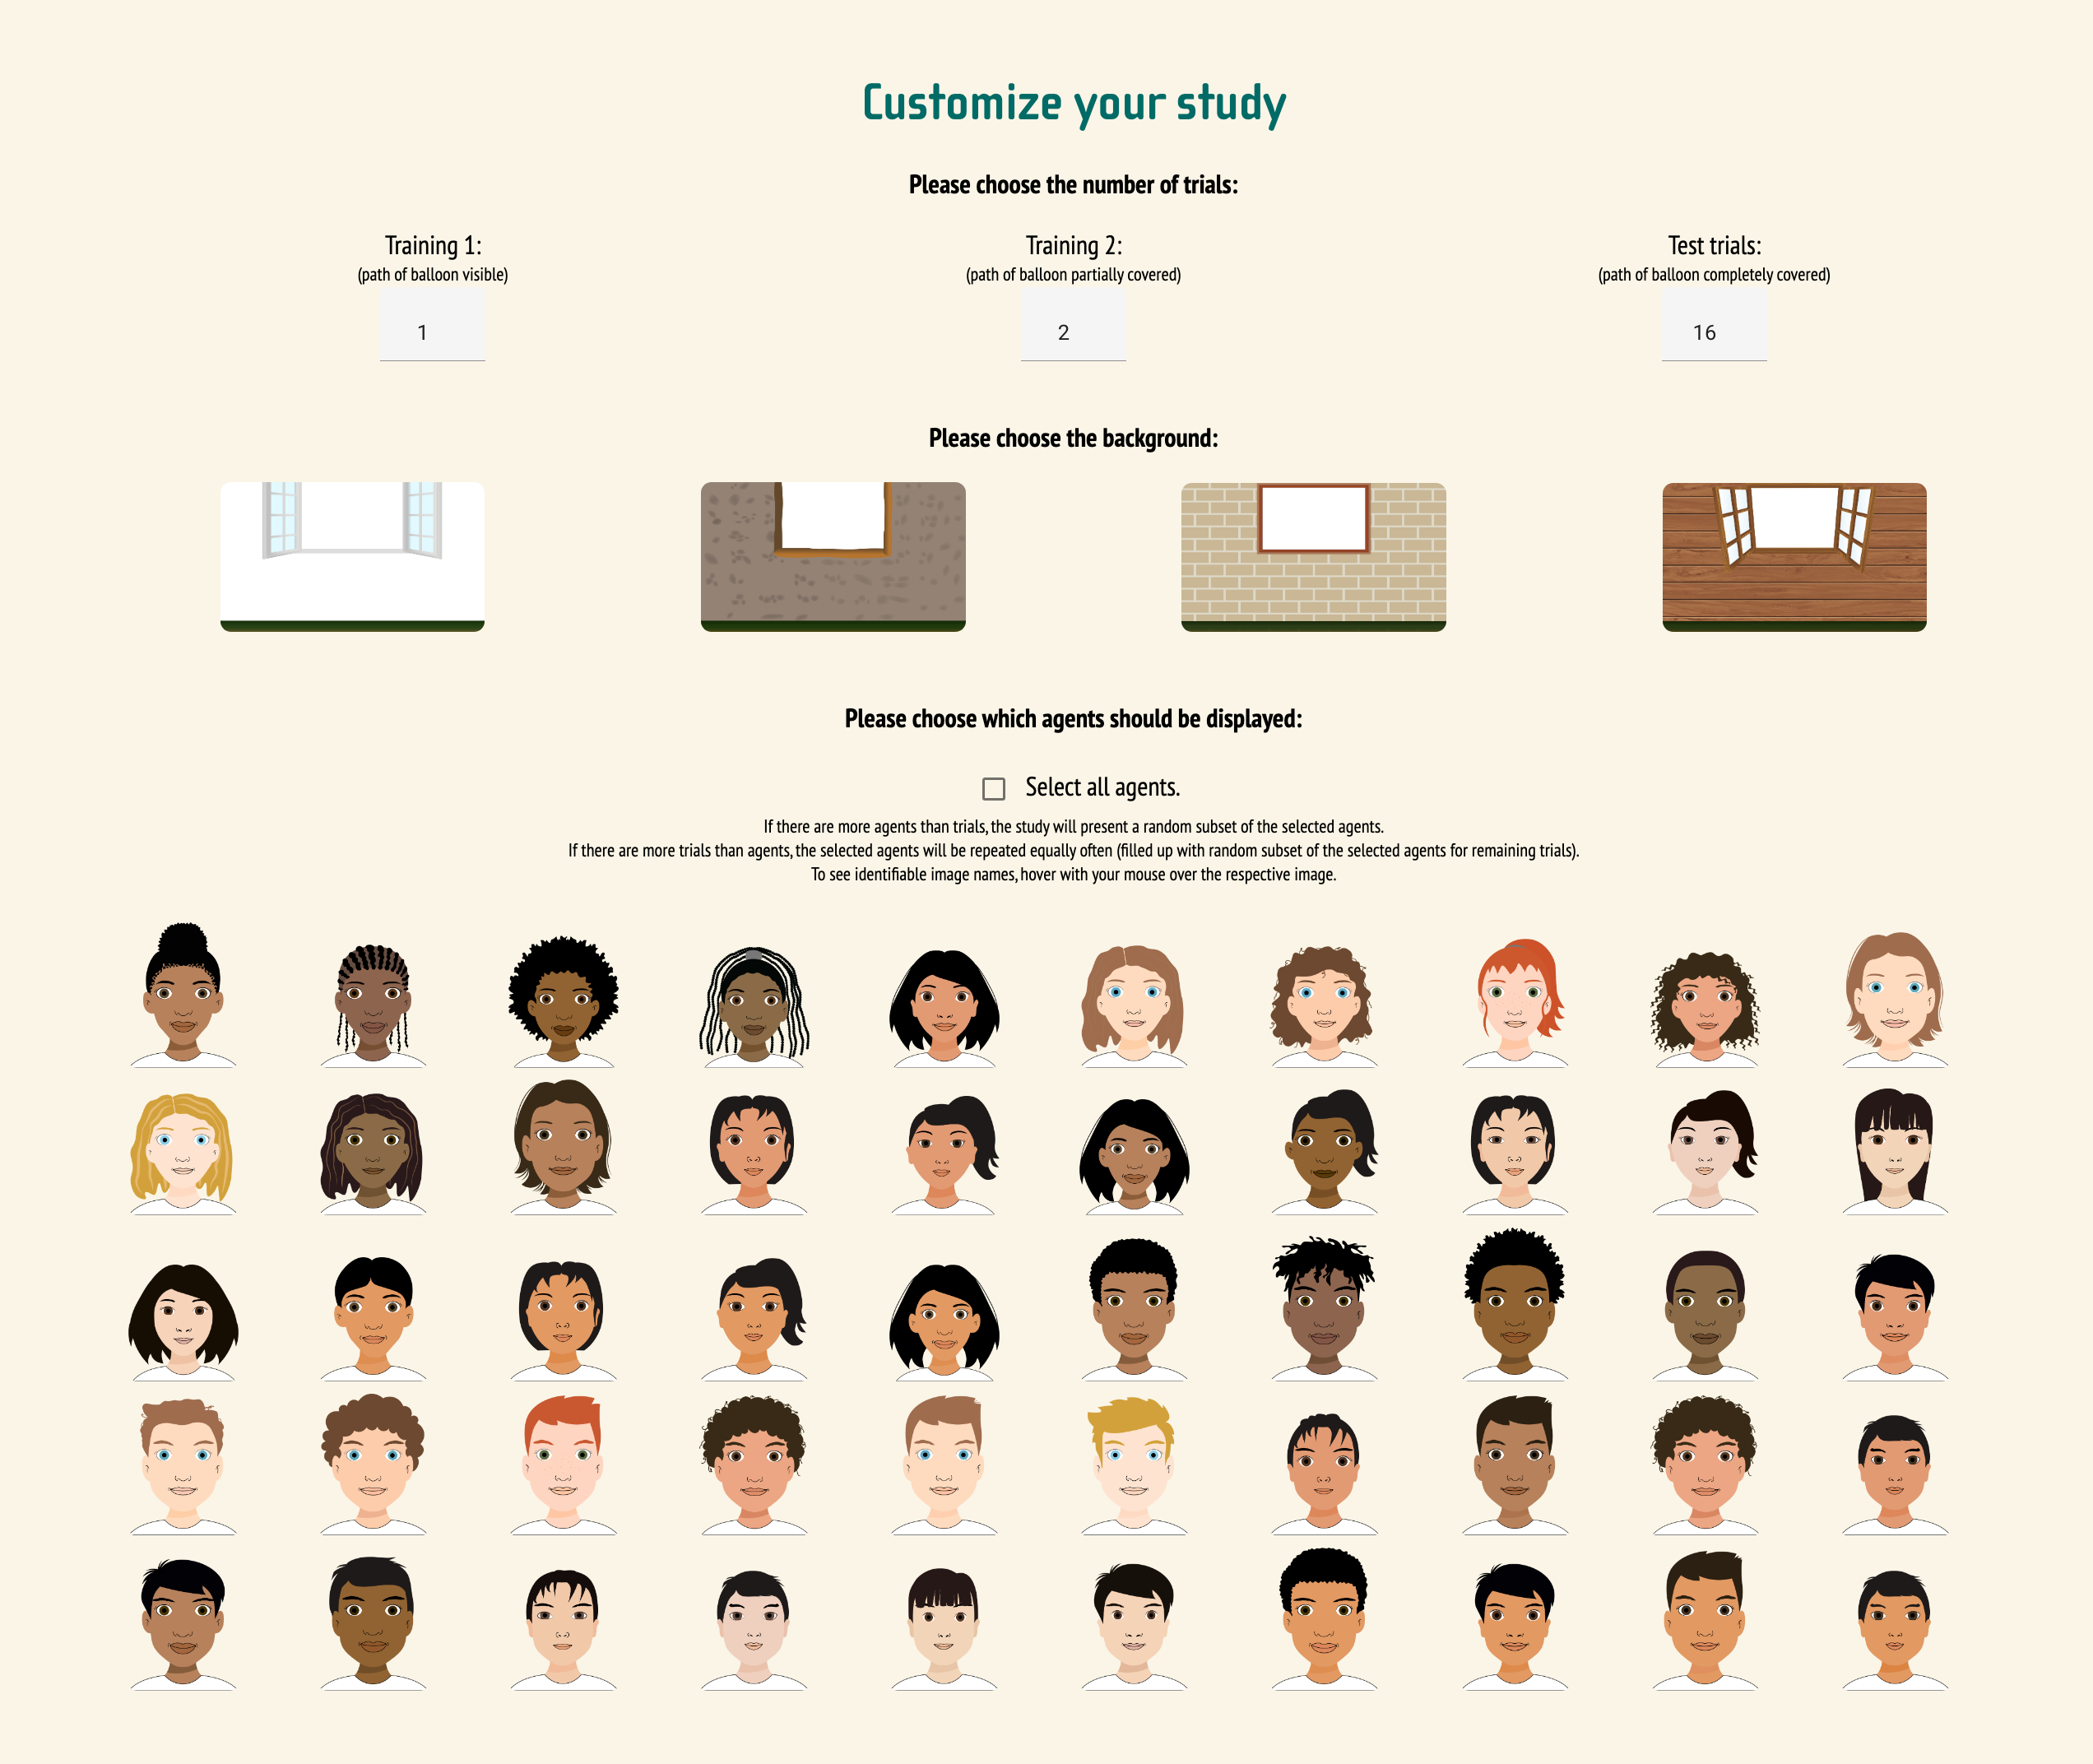
\includegraphics[width=1\linewidth]{../figures/tango-cc-screenshot} 

}

\caption{\textbf{Screenshot of the customizable components of the TANGO-CC.} Researchers can select the language of the audio instructions (see Table 1), the number of trials per trial type, the background, and the agent's face.}\label{fig:fig2}
\end{figure}

\subsubsection{Task implementation}\label{task-implementation}

The task was implemented in \texttt{JavaScript}, \texttt{HTML}, and \texttt{CSS} and is presented as a web app.
It can be accessed on any modern web browser on any device (e.g., computer or tablet) and does not require prior installation (though please note that configurations of browsers and JavaScript may change in the future).
Participant's responses can be recorded on a touchscreen or with a mouse or trackpad.
The online version of the task can be used for unsupervised data collection (for example, using online platforms like \emph{Prolific}; see Prein, Kalinke, et al. (2024)). The task can be shared easily internationally by providing the URL.
Importantly, the web app implementation does not require a working WIFI connection: An offline version of the task can be downloaded and quickly set up for devices that support Node.js (\url{https://nodejs.org/en}).
This is an especially useful feature for researchers working in locations with limited internet access.

The stimuli are embedded as Scalable Vector Graphics (SVG; an XML format that describes elements in mathematical formulas based on points and lines on a grid).
SVGs ensure that the picture quality, aspect ratio, and relative object positioning are constant.
Furthermore, stimuli are added as individual components to the image scene which allows for an easy adaptation of the task's elements (in contrast to other image formats that consist of only one combined layer that would need entire replacement).
The task is programmed so that responses are only registered when the participant clicks the relevant part of the screen (i.e., in test trials, when they click the hedge).
Furthermore, clicks are only registered after the voice recordings stop playing.
An audio reminder is played again if no click is registered within 5 seconds.

The website does not use cookies, nor does it upload any data to servers; that is, the data is only stored locally on the device.
The output of the task is a CSV file (and WEBM file if a webcam recording was selected) that contains the participants' responses and can be easily imported into statistical software for further analysis.
The file will be stored in the device's downloads folder and is named after the following pattern: ``tangoCC-participantID-YYYY-MM-DD\_hh\_mm\_ss''. To modify the storage location on the device, researchers can change the designated downloads folder in their browser settings.

\section{Psychometric evaluation}\label{psychometric-evaluation}

\subsection{Data set}\label{data-set}

We used the data set from Bohn, Prein, et al. (2024) for the psychometric evaluation of the TANGO-CC.
The data set contains a sample of \emph{N} = 1377 children, aged 2.5 to 11 years (see supplements).
Participants came from 17 communities on five continents, in rural and urban settings, with varying degrees of market integration and technology exposure.
Bohn, Prein, et al. (2024) carried out 19 trials (1 training 1, 2 training 2, and 16 test trials, of which the first of each type had audio instructions) on a touchscreen device.
Faces, backgrounds, and languages were chosen by researchers and assistants with experience in the specific community.
For further details on the communities, participant information, and data collection procedures, see the supplements of Bohn, Prein, et al. (2024).

\subsection{Individual differences}\label{individual-differences}



\begin{figure}

{\centering 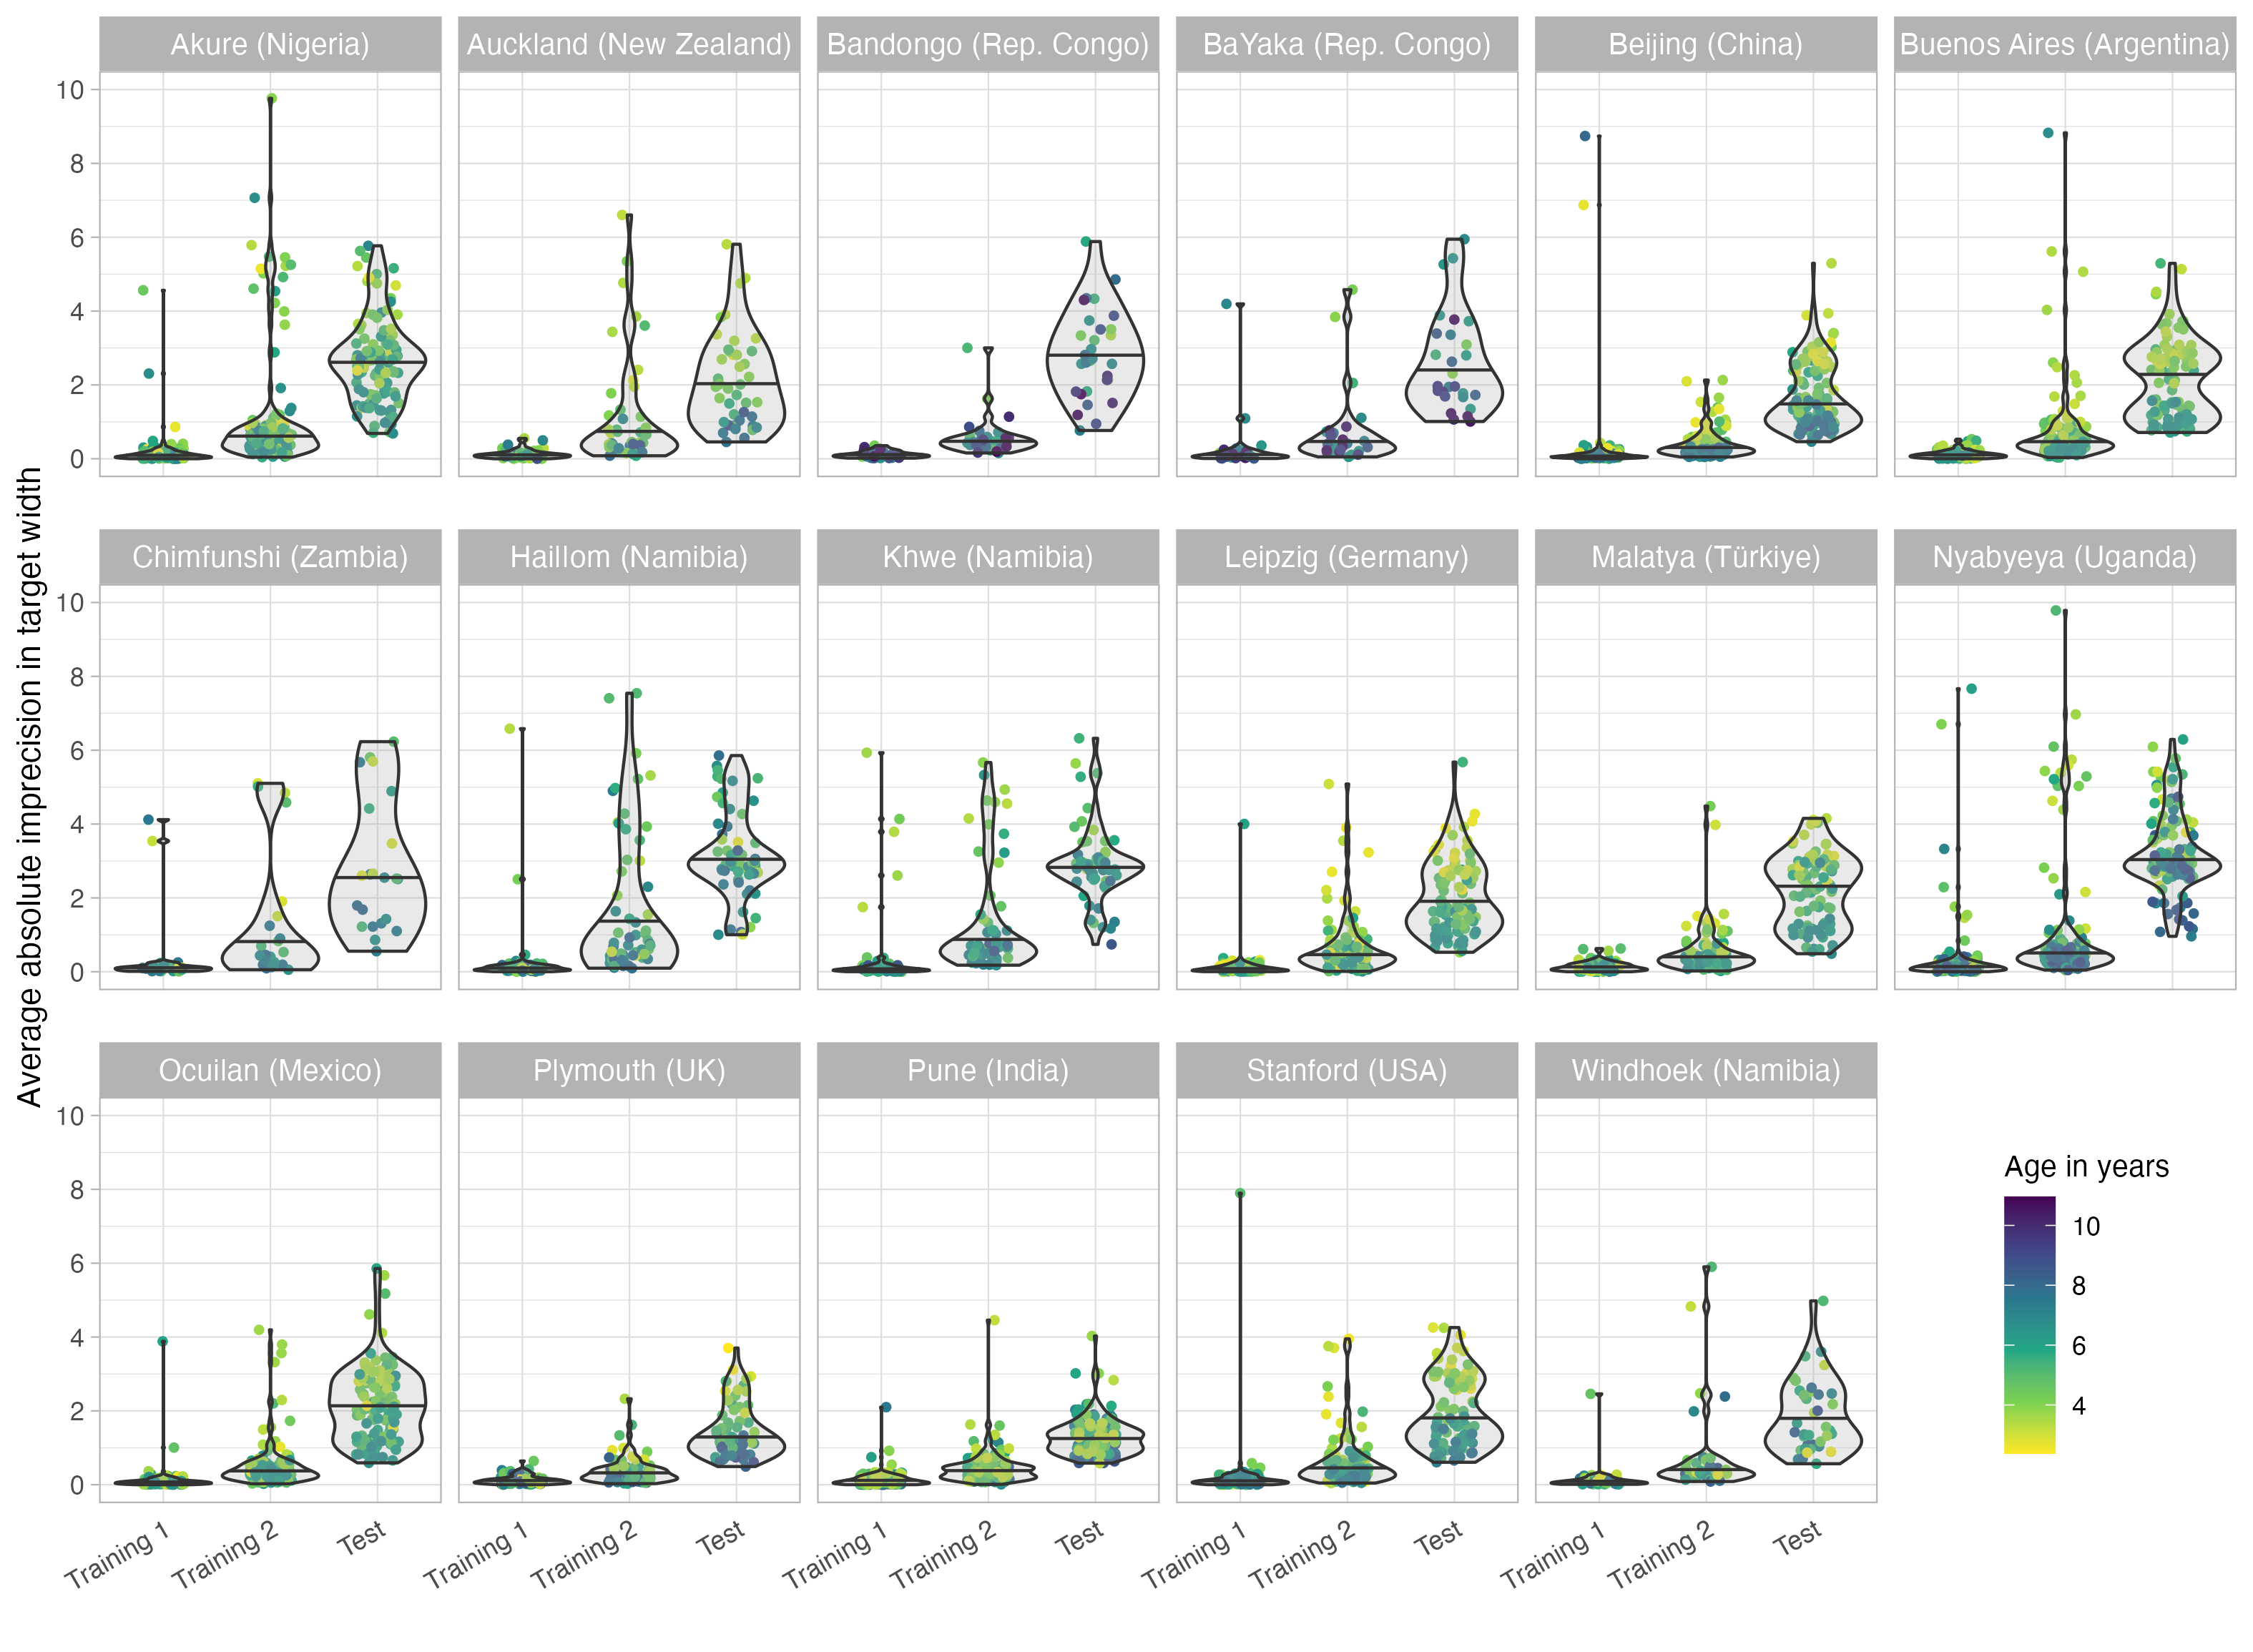
\includegraphics[width=1\linewidth]{../figures/tango-cc-variability} 

}

\caption{\textbf{Variability measured by the TANGO-CC.} Mean imprecision in locating the agent's attentional focus by community (alphabetically) and trial type. Imprecision is defined as the distance between the participant's click and the balloon's center in units of balloon width. For a depiction of each trial's procedure, see Figure \ref{fig:fig1}.}\label{fig:fig3}
\end{figure}

All analyses and the data set can be accessed on GitHub (\url{https://github.com/ccp-eva/tango-cc-methods/}).
First, we inspected the mean and standard deviations by community and compared performance in each trial type (training 1, training 2, test trials).
Performance was defined as the absolute distance between the target center and the x coordinate of the participant's click (measured in balloon widths).
Across communities, children performed best in training 1 (mean = 0.19, sd = 0.63), followed by training 2 (mean = 0.79, sd = 1.44) and test trials (mean = 2.21, sd = 2.03; see Figure \ref{fig:fig3}).

To formally estimate the effect of trial type on performance in the TANGO-CC, we fitted a generalized linear mixed model (GLMM) predicting the task performance by trial type (reference category: test trials).
All analyses were run in R version 4.4.1 (2024-06-14) (R Core Team, 2024).
GLMMs were fitted with default priors using the function \texttt{brm} from the package \texttt{brms} (Bürkner, 2017, 2018).
The model included random effects for trial type by community (model notation in \texttt{R:\ imprecision\ \textasciitilde{}\ trialtype\ +\ (trialtype\ \textbar{}\ community)}), and imprecision was modeled by a \texttt{lognormal} distribution.
We inspected the posterior distribution (mean and 95\% Credible Interval (CrI)) for the trial type estimates.

Our GLMM analysis supported the visual inspection of the data: the fixed-effect estimates for training 1 (\(\beta\) = -3.26; 95\% CrI {[}-3.41; -3.10{]}) and training 2 (\(\beta\) = -1.47; 95\% CrI {[}-1.58; -1.35{]}) were negative and reliably different from zero.\footnote{Please note that the TANGO-CC measures imprecision in gaze following.
  Therefore, a negative sign indicates that children showed less imprecision (i.e., were more precise) in the training trials than in the test trials.}
This effect was found across all communities (random effects of trial type within community: minimum estimate for training 1 = -2.87; 95\%CrI {[}-3.11; -2.60{]}; minimum estimate for training 2 = -1.27; 95\%CrI {[}-1.51; -0.98{]}).
The almost perfect performance in training trials indicated that children understood the task and were able to correctly indicate the location of the balloon when its path was (mostly) visible.
In test trials, children's imprecision was higher, indicating that the task was more challenging.
All communities showed substantial individual variation and overlapped in their imprecision levels (see Figure \ref{fig:fig3}).

To identify the sources of variation, we computed intraclass correlations (ICC).
The variation in children's imprecision within communities was substantially larger than the variation between the communities.
The mean within-community variance was 1.28, ranging from 0.24 (in Pune, India) to 3.46 (in Chimfunshi, Zambia).
Between-community variance was 0.34.
The ICC, representing the proportion of between-community variance relative to the total variance (sum of within- and between-community variance), was 0.02.
This indicated that only 2\% of the total variability in the data could be attributed to differences between communities, while the remaining 98\% were attributed to differences within communities (Kusano et al., 2024).

\subsection{Reliability}\label{reliability}



\begin{figure}

{\centering 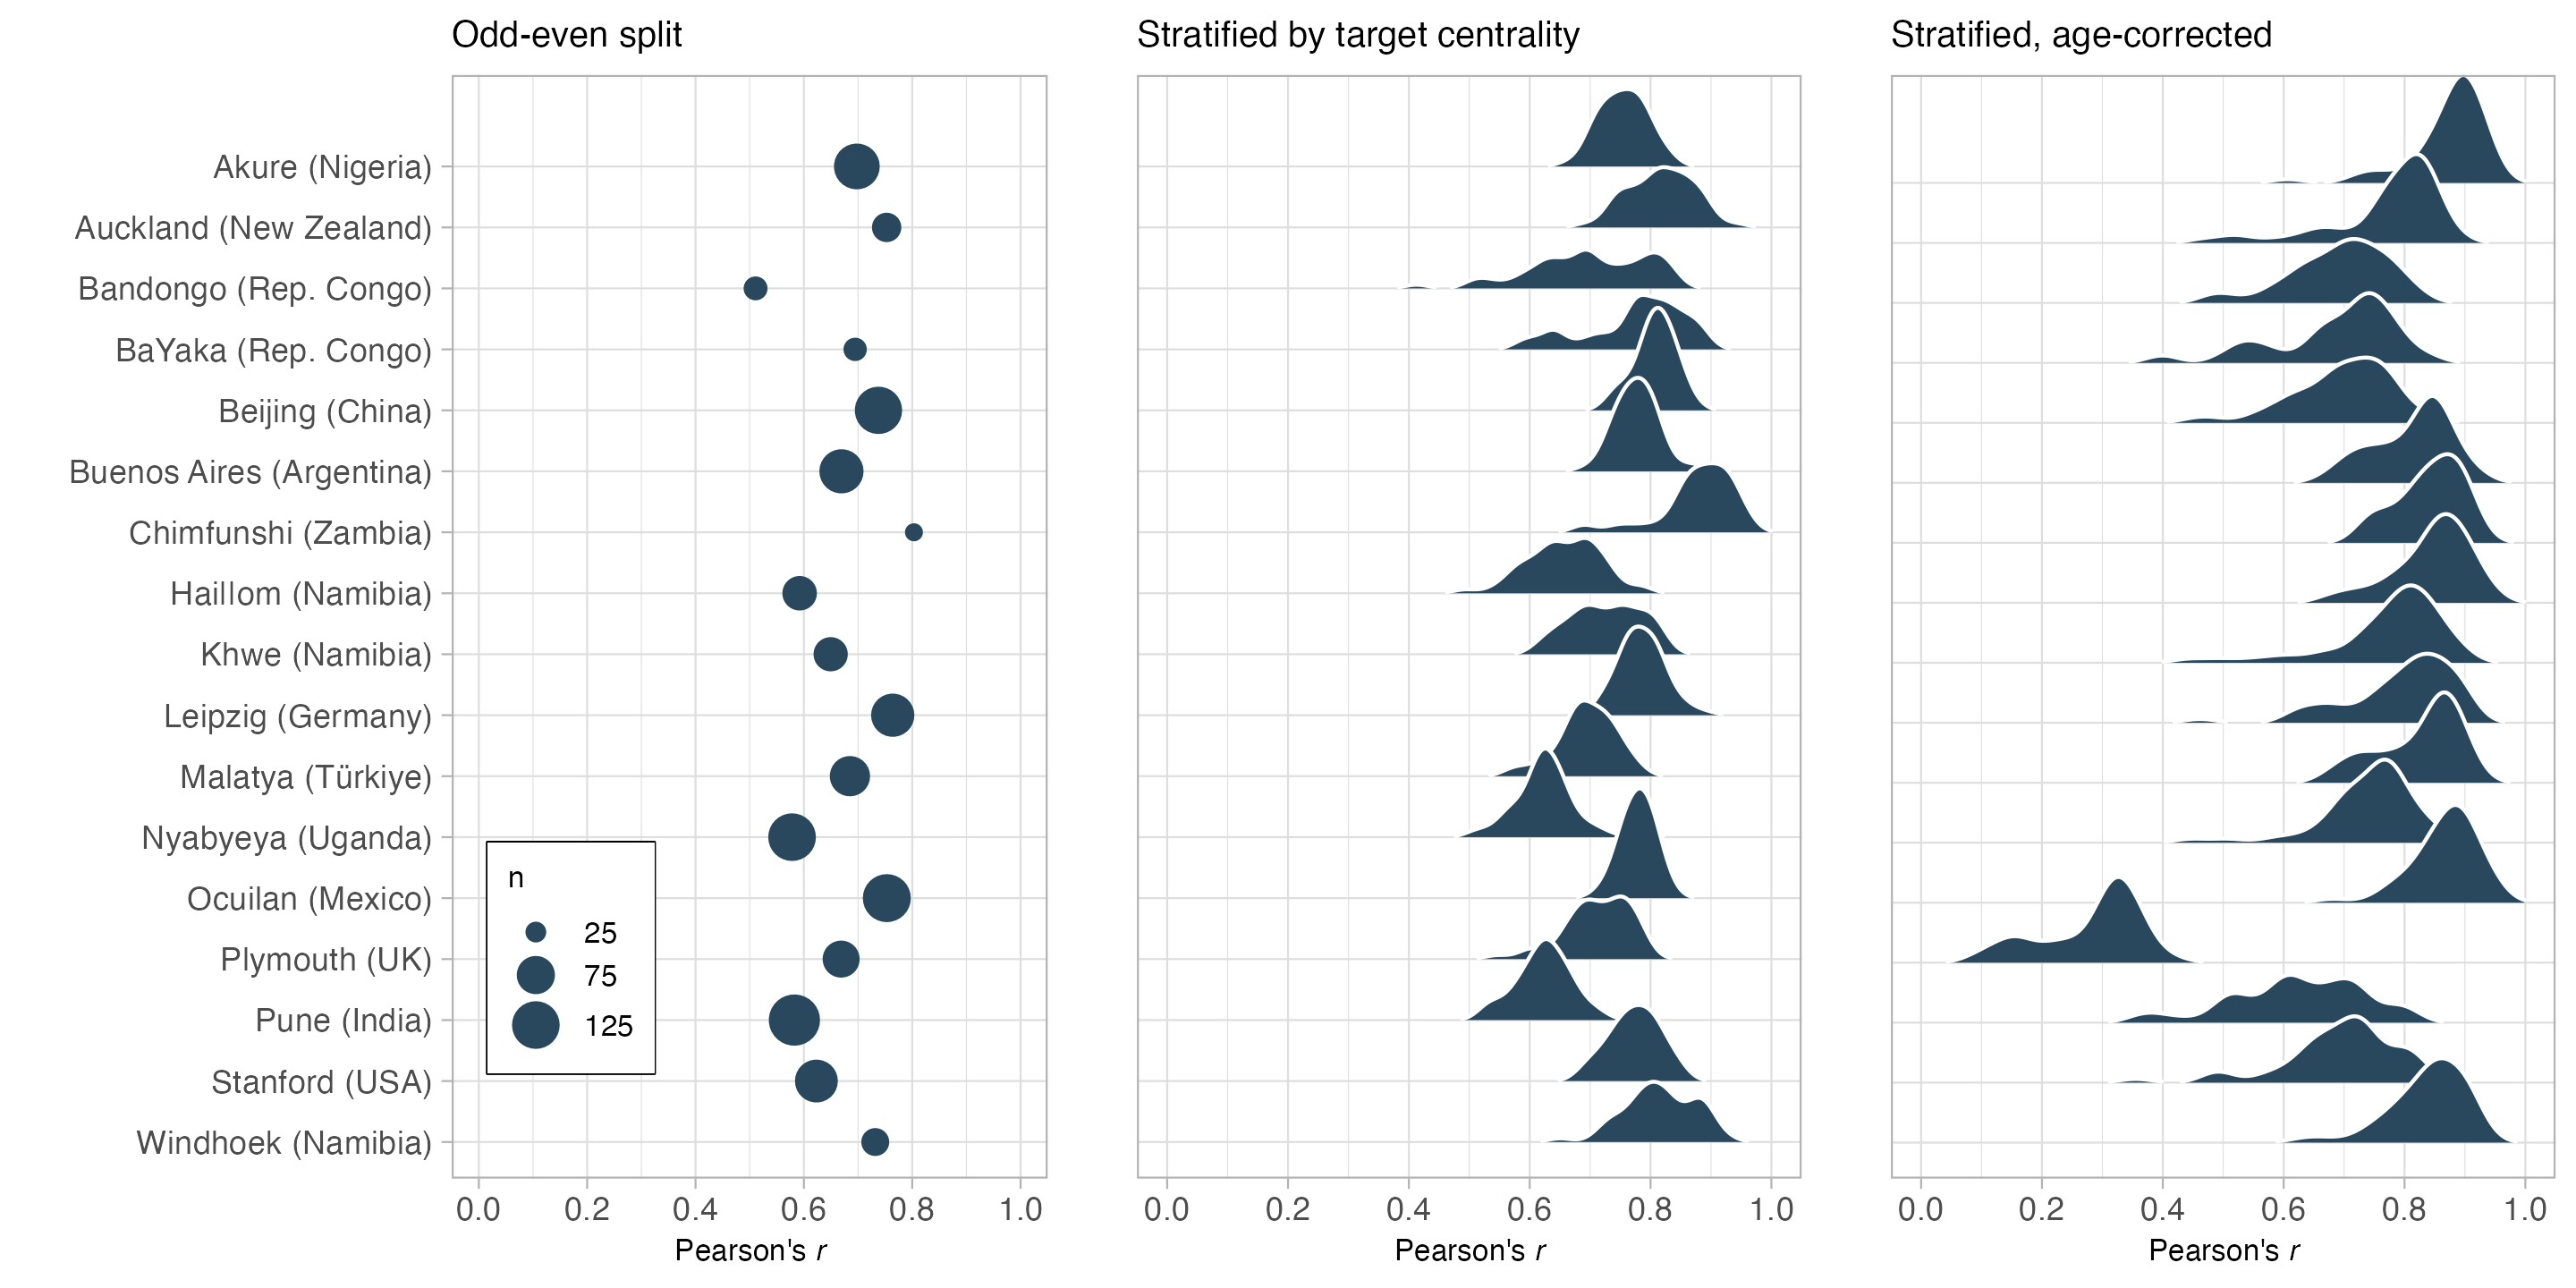
\includegraphics[width=1\linewidth]{../figures/tango-cc-reli} 

}

\caption{\textbf{Reliability of the TANGO-CC by community.} Internal consistency estimates by community, following three different approaches. In the odd-even split, the size of points reflects the sample size in each community. In the stratified approach with and without age correction, density curves show the posterior distributions of the GLMM.}\label{fig:fig4}
\end{figure}

To assess reliability, we estimated internal consistency in each community in three different ways.
First, data of each participant was split into odd and even trials and a Pearson correlation was calculated between the aggregated scores of the two halves.
Second, using the function \texttt{by\_split} from the \texttt{splithalfr} package (Pronk et al., 2022), data was stratified by target centrality, and a Pearson correlation was calculated between the matched halves.
Target centrality measured how closely the target landed to the center of the screen (i.e., distance from the balloon center to the screen center), which served as a proxy for trial difficulty and was previously found to be a relevant component in predicting participants' performance in a cognitive model (Prein, Maurits, et al., 2024).
Third, a data set was generated with stratified test halves by target centrality and we applied the GLMM approach introduced by Rouder and Haaf (2019).
A GLMM was fitted with the mean imprecision as the outcome, age as the predictor, and test half and participant id as random effects (model notation: \texttt{imprecision\ \textasciitilde{}\ age\ +\ (0\ +\ half\ \textbar{}\ subjid)}).
The model estimates correlations between participant-specific estimates for each test half.
The hierarchical shrinkage of the model enables accurate person-specific estimates.
By incorporating age as a fixed effect, the correlation between the two person-specific estimates represents the age-independent estimate for internal consistency.
This removes the possibility that a good internal consistency estimate results from general cognitive development rather than task-specific inter-individual differences.
Because the process of generating stratified data sets is partly random, the model was fitted 50 times for each community.
The posterior estimate of the correlation between the two person-specific estimates was taken as the age-independent estimate for internal consistency.

The results are shown in Figure \ref{fig:fig4}.
Across communities, internal consistency estimates ranged from 0.51 to 0.80 for the odd-even split, 0.62 to 0.89 for the stratified internal consistency, and 0.62 to 0.87 for the age-corrected approach (Plymouth, UK, being an outlier with 0.28).
Following Cohen's suggestions (Cohen, 1988, 1992), these correlations constitute large effects (\emph{r} \textgreater{} .50), and indicate good internal consistency.\footnote{Note that for scale reliability and Cronbach's \(\alpha\), values of .7 to .8 have been suggested to be acceptable (Field et al., 2012; Kline, 1999). However, Kline (1999) suggested that values below .7 could be realistic for psychological constructs due to their variable nature.}
The results are comparable to the internal consistency estimates found in the original TANGO study (Prein, Kalinke, et al., 2024), and also resemble reliability estimates of classical false belief tasks (Hughes et al., 2000).

In an exploratory analysis, we found that communities with larger individual variation showed higher internal consistency estimates (Pearson's \emph{r} = 0.46, 95\%CI {[}-0.03; 0.77{]}).
This suggests that the less variation a task can capture within a community, the lower the reliability.
However, please note that this correlation could be influenced by outliers and that the sample size here (\emph{N} = 17 communities) is too small to make substantial claims.

\section{Discussion}\label{discussion}

The TANGO-CC measures imprecision in gaze following across individuals, ages, and communities.
Children's imprecision in gaze following showed highly similar result patterns across communities: children performed better in the training than the test trials, and within-community variation greatly exceeded between-community variation.
Furthermore, the task showed satisfactory to high reliability across all communities.
Therefore, the TANGO-CC is a suitable task to capture individual differences in social-cognitive development in diverse communities.

The TANGO-CC's design process lays out a much-needed pragmatic approach to studying community-level and individual-level differences across cultures:
While we performed a detailed psychometric evaluation of the task in a German setting, we collaborated with local researchers for the cross-cultural stimulus development and selection.
Importantly, we re-assessed the TANGO-CC's psychometric properties in a large and diverse data set.
While we cannot generalize our findings to all communities worldwide, we found that the TANGO-CC captured reliable individual variation in all 17 communities studied by Bohn, Prein, et al. (2024).
We hope that not just the TANGO-CC but also our pragmatic approach to constructing it will be helpful to other researchers.
We recommend that researchers consider generalizability concerns and cross-cultural applications of their tasks and collaborate with local researchers at the early stages of task development (Torréns et al., 2023).
Using the TANGO-CC (or any other task) in a new community requires sensitivity to the specific context, piloting, and, most importantly, the involvement of researchers or research assistants from the specific community.

Bourdage et al. (2023) pointed out a major challenge with adapting social cognition tasks to diverse communities: the number of world cultures is vast, and communities are constantly changing.
Therefore, a promising approach might be to provide tasks with a modular system where components can be modified (i.e., building block structure).
In the case of the TANGO-CC, the task cannot only be adapted to different languages, cartoon faces, and backgrounds (see Figure \ref{fig:fig2}) but also updated with new stimuli.
Unlike studies that present sequential, hand-painted pictures that are difficult to adapt (Mehta et al., 2011), the TANGO-CC uses SVGs (Scalable Vector Graphics) that can be easily exchanged.

Compared to one of the most commonly used social cognition measures -- the change-of-location false belief task (Baron-Cohen et al., 1985; Wimmer \& Perner, 1983) -- the TANGO-CC has several advantages: a continuous outcome measure that can capture individual differences from three years to adulthood, a short task duration that allows for more trials per child, stimuli that can be easily adapted, and known psychometric properties across 17 communities.
The task is presented as a web app that enables efficient data collection with large sample sizes, while it can also be used to collect data offline in locations without a reliable internet connection.
The TANGO-CC follows a standardized procedure, which prevents rater errors and greatly simplifies online training of research assistants.
Furthermore, minimal language demands and an engaging, playful design increase the task's usability and reduce non-completion rates.

The TANGO-CC will be a useful asset for exploring a range of research questions.
First, the TANGO-CC could be applied to assessing relationships between gaze following and other (social-) cognitive constructs. Examples include the relationship between gaze following and Theory of Mind (Prein, Maurits, et al., 2024) or eye gaze in sharing behaviors and Dictator games (Kelsey et al., 2018; Manesi et al., 2016; Nettle et al., 2013; Wu et al., 2018). Second, the TANGO-CC could be used to examine the influence of environmental factors on gaze following. Environmental factors of interest could include household size (Bohn, Fong, et al., 2024) or maternal postpartum depression (Astor et al., 2022). Third, scores in the TANGO-CC could predict performance in other tasks at later time points. This would be helpful for assessing predictive validity of gaze following, for example for language comprehension (Prein, Kalinke, et al., 2024). Fourth, the TANGO-CC could be applied to measure children's gaze following development longitudinally, potentially combined with interim interventions. The task is suitable for children, teenagers, and adults alike and is sensitive to individual differences throughout the lifespan (established in a German sample; Prein, Kalinke, et al. (2024)).

The TANGO-CC is a screen-based task.
Bohn, Prein, et al. (2024) have shown that children with no prior touchscreen exposure were less precise in the TANGO-CC than children with prior experience.
Therefore, the mode of stimulus presentation needs to be kept in mind when administering the TANGO-CC, especially in communities with little technology exposure.
Additional touchscreen training (e.g., more trials of training 1) might prove helpful in these cases.
If researchers are interested in controlling for an effect of stimulus presentation, we recommend gathering information on touchscreen exposure.

Interestingly, individual differences were also present in communities with 100\% touchscreen exposure, showing that this factor alone could not explain children's performance in the task (Bohn, Prein, et al., 2024).
Even though the touchscreen experience caused absolute differences in task performance, all communities showed the same processing signature: Children were more precise in trials in which the agent looked to a more central position (i.e., higher target centrality) compared to a position to the far left or right of the screen.
A computational cognitive model predicted this processing signature and described gaze following as a process of estimating pupil angles and the corresponding gaze vectors (Prein, Maurits, et al., 2024).
Bohn, Prein, et al. (2024) found clear support for this model in every community studied, suggesting that children all over the world process gaze in a similar way.
Alternative theories on gaze following exist, but have not been cross-culturally validated to date.
Doherty et al. (2015) proposed two separate gaze processing systems based on luminance versus geometric cues.
Other theoretical accounts assign a central role to reinforcement learning (Corkum \& Moore, 1998; Ishikawa et al., 2020; Silverstein et al., 2021; Triesch et al., 2006) or self-other equivalence (``like me'', Meltzoff (2007), Meltzoff (2005)).

Schilbach et al. (2013) pointed out that witnessing social interactions as an observer undoubtedly differs from actively participating in social interactions.
First evidence suggests that the TANGO-CC indeed taps into social cognition as utilized in real life: Prein, Maurits, et al. (2024) found that children's perspective-taking abilities in a personal social interaction were linked to performance in the TANGO, but less so to a matched, non-social vector following task.
However, this study exclusively relied on a German sample and future research should investigate whether the relationship between the TANGO-CC and perspective-taking abilities holds across communities.

We have reported reliability estimates for each community by calculating internal consistency.
Ideally, we would have additionally evaluated the task's test-retest reliability in each community and checked for relationships with theoretically related constructs to assess validity.
Unfortunately, this might not always be feasible in large-scale cross-cultural studies due to organizational and financial constraints.
An example of assessing the TANGO's predictive validity is a study conducted in Leipzig, Germany, which used the TANGO to predict children's receptive vocabulary 6 months later (Prein, Kalinke, et al., 2024).
Future cross-cultural studies could investigate the TANGO-CC's predictive validity and its relationship to other social-cognitive abilities (e.g., Theory of Mind, language development) in diverse communities.

Measurement invariance (i.e., measuring the same construct across different communities) is often seen as a requirement for a ``fair'' cross-cultural comparison: it is important that any group differences are not the result of the task unintentionally tapping into different underlying constructs.
As Kusano et al. (2024) put it: ``The research challenge is to achieve a balance between ensuring methodological ``fairness'' at the individual level while also recognizing and capturing genuine sociocultural variability'' (p.~34).
We argue that the TANGO-CC measures a fundamental social-cognitive ability that is likely similar across communities.
Selcuk et al. (2023) pointed out that researchers should study both within- and between-culture variability in the development of social cognition since sometimes within-culture differences exceed between-culture differences.
Indeed, we found that within-group variability was greater than between-group variability.
While we believe that the TANGO-CC can be used to compare mean differences across communities, we would recommend using it to study individual differences within communities.

For years, researchers have called for more diverse sampling and culturally valid measures of cognitive development (Matsumoto \& Yoo, 2006; e.g., Mehta et al., 2011; Nielsen et al., 2017).
As Hajdúk et al. (2020) said, ``using large samples and multisite approaches will align with efforts to improve reproducibility {[}replicability{]} and will clarify both the type and extent of cultural influences on social cognition'' (p.~463).
Similarly, Elson et al. (2023) have called for standardized, psychometrically evaluated measures that can be re-used by other researchers in order to ``build a cumulative evidence base in psychology'' (p.~2).
This underlines how efforts to improve replicability can be combined with the goal of increasing the generalisability of psychological research findings (Li et al., 2024; Syed, 2021).
Li et al. (2024) have argued that replicable and generalizable results rely on stimulus sets with slight variations, more diverse samples, and data collection at a greater scale, which are indeed all steps the TANGO-CC has taken.
Openly sharing the TANGO-CC's materials will allow other researchers to (hopefully) replicate the results and deepen our cumulative understanding of social-cognitive development across diverse communities.

\section{Conclusion}\label{conclusion}

The TANGO-CC captures individual differences in social-cognitive development across diverse communities.
The task's customizability, minimal language demands, and its efficient data collection method make it a valuable tool for cross-cultural research.
The task showed satisfactory to high reliability (internal consistency) in a large data set including 17 diverse communities on five continents.
We hope that the TANGO-CC -- and its pragmatic construction process -- will provide a roadmap for future cross-cultural studies on cognitive development.

\newpage

\section{References}\label{references}

\begingroup
\setlength{\parindent}{-0.5in}
\setlength{\leftskip}{0.5in}

\phantomsection\label{refs}
\begin{CSLReferences}{1}{0}
\bibitem[\citeproctext]{ref-adolphs1999social}
Adolphs, R. (1999). Social cognition and the human brain. \emph{Trends in Cognitive Sciences}, \emph{3}(12), 469--479. \url{https://doi.org/10.1016/S1364-6613(99)01399-6}

\bibitem[\citeproctext]{ref-akhtar2008privileging}
Akhtar, N., \& Gernsbacher, M. A. (2008). On {Privileging} the {Role} of {Gaze} in {Infant Social Cognition}. \emph{Child Development Perspectives}, \emph{2}(2), 59--65. \url{https://doi.org/10.1111/j.1750-8606.2008.00044.x}

\bibitem[\citeproctext]{ref-amir2020crosscultural}
Amir, D., \& McAuliffe, K. (2020). Cross-cultural, developmental psychology: Integrating approaches and key insights. \emph{Evolution and Human Behavior}, \emph{41}(5), 430--444. \url{https://doi.org/10.1016/j.evolhumbehav.2020.06.006}

\bibitem[\citeproctext]{ref-anderson1997preschoolers}
Anderson, J. R., \& Doherty, M. J. (1997). Preschoolers' perception of other people's looking: {Photographs} and drawings. \emph{Perception}, \emph{26}(3), 333--343. \url{https://doi.org/10.1068/p260333}

\bibitem[\citeproctext]{ref-apicella2020weird}
Apicella, C., Norenzayan, A., \& Henrich, J. (2020). Beyond {WEIRD}: {A} review of the last decade and a look ahead to the global laboratory of the future. \emph{Evolution and Human Behavior}, \emph{41}(5), 319--329. \url{https://doi.org/10.1016/j.evolhumbehav.2020.07.015}

\bibitem[\citeproctext]{ref-arnett2008neglecteda}
Arnett, J. J. (2008). The neglected 95\%: {Why American} psychology needs to become less {American}. \emph{American Psychologist}, \emph{63}(7), 602--614. \url{https://doi.org/10.1037/0003-066X.63.7.602}

\bibitem[\citeproctext]{ref-astor2022gaze}
Astor, K., \& Gredebäck, G. (2022). Gaze following in infancy: {Five} big questions that the field should answer. In \emph{Advances in {Child Development} and {Behavior}} (Vol. 63, pp. 191--223). Elsevier. \url{https://doi.org/10.1016/bs.acdb.2022.04.003}

\bibitem[\citeproctext]{ref-astor2022maternal}
Astor, K., Lindskog, M., Juvrud, J., Wangchuk, Namgyel, S. C., Wangmo, T., Tshering, K., \& Gredebäck, G. (2022). Maternal postpartum depression impacts infants' joint attention differentially across cultures. \emph{Developmental Psychology}, \emph{58}(12), 2230--2238. \url{https://doi.org/10.1037/dev0001413}

\bibitem[\citeproctext]{ref-baron-cohen1985does}
Baron-Cohen, S., Leslie, A. M., \& Frith, U. (1985). Does the autistic child have a "theory of mind" ? \emph{Cognition}, \emph{21}, 37--46. \url{https://doi.org/10.1016/0010-0277(85)90022-8}

\bibitem[\citeproctext]{ref-beaudoin2020systematic}
Beaudoin, C., Leblanc, É., Gagner, C., \& Beauchamp, M. H. (2020). Systematic {Review} and {Inventory} of {Theory} of {Mind Measures} for {Young Children}. \emph{Frontiers in Psychology}, \emph{10}, 2905. \url{https://doi.org/10.3389/fpsyg.2019.02905}

\bibitem[\citeproctext]{ref-bohn2024understanding}
Bohn, M., Fong, F. T. K., Pope-Caldwell, S., Stengelin, R., \& Haun, D. B. M. (2024). Understanding cultural variation in cognition one child at a time. \emph{Nature Reviews Psychology}. \url{https://doi.org/10.1038/s44159-024-00351-8}

\bibitem[\citeproctext]{ref-bohn2018common}
Bohn, M., \& Köymen, B. (2018). Common {Ground} and {Development}. \emph{Child Development Perspectives}, \emph{12}(2), 104--108. \url{https://doi.org/10.1111/cdep.12269}

\bibitem[\citeproctext]{ref-bohn2024universal}
Bohn, M., Prein, J. C., Ayikoru, A., Bednarski, F. M., Dzabatou, A., Frank, M. C., Henderson, A. M. E., Isabella, J., Kalbitz, J., Kanngiesser, P., Keşşafoğlu, D., Koymen, B., Manrique-Hernandez, M., Magazi, S., Mújica-Manrique, L., Ohlendorf, J., Olaoba, D., Pieters, W., Pope-Caldwell, S., \ldots{} Haun, D. (2024). \emph{A universal of human social cognition: {Children} from 17 communities process gaze in similar ways}. PsyArXiv. \url{https://doi.org/10.31234/osf.io/z3ahv}

\bibitem[\citeproctext]{ref-bourdage2023evaluation}
Bourdage, R., Narme, P., Neeskens, R., Papma, J., \& Franzen, S. (2023). An {Evaluation} of {Cross-Cultural Adaptations} of {Social Cognition Testing}: {A Systematic Review}. \emph{Neuropsychology Review}. \url{https://doi.org/10.1007/s11065-023-09616-0}

\bibitem[\citeproctext]{ref-broesch2023roadmap}
Broesch, T., Lew-Levy, S., Kärtner, J., Kanngiesser, P., \& Kline, M. (2023). A roadmap to doing culturally grounded developmental science. \emph{Review of Philosophy and Psychology}, \emph{14}(2), 587--609. \url{https://doi.org/10.1007/s13164-022-00636-y}

\bibitem[\citeproctext]{ref-brooks2005development}
Brooks, R., \& Meltzoff, A. N. (2005). The development of gaze following and its relation to language. \emph{Developmental Science}, \emph{8}(6), 535--543. \url{https://doi.org/10.1111/j.1467-7687.2005.00445.x}

\bibitem[\citeproctext]{ref-brooks2015connecting}
Brooks, R., \& Meltzoff, A. N. (2015). Connecting the dots from infancy to childhood: {A} longitudinal study connecting gaze following, language, and explicit theory of mind. \emph{Journal of Experimental Child Psychology}, \emph{130}, 67--78. \url{https://doi.org/10.1016/j.jecp.2014.09.010}

\bibitem[\citeproctext]{ref-brooks2020enhanced}
Brooks, R., Singleton, J. L., \& Meltzoff, A. N. (2020). Enhanced gaze-following behavior in {Deaf} infants of {Deaf} parents. \emph{Developmental Science}, \emph{23}(2), e12900. \url{https://doi.org/10.1111/desc.12900}

\bibitem[\citeproctext]{ref-burkner2017brms}
Bürkner, P.-C. (2017). Brms: {An R Package} for {Bayesian Multilevel Models Using Stan}. \emph{Journal of Statistical Software}, \emph{80}(1), 1--28. \url{https://doi.org/10.18637/jss.v080.i01}

\bibitem[\citeproctext]{ref-burkner2018advanced}
Bürkner, P.-C. (2018). Advanced {Bayesian Multilevel Modeling} with the {R Package} brms. \emph{The R Journal}, \emph{10}(1), 395. \url{https://doi.org/10.32614/RJ-2018-017}

\bibitem[\citeproctext]{ref-butler2000infant}
Butler, S. C., Caron, A. J., \& Brooks, R. (2000). Infant {Understanding} of the {Referential Nature} of {Looking}. \emph{Journal of Cognition and Development}, \emph{1}(4), 359--377. \url{https://doi.org/10.1207/S15327647JCD0104_01}

\bibitem[\citeproctext]{ref-callaghan2011early}
Callaghan, T., Moll, H., Rakoczy, H., Warneken, F., Liszkowski, U., Behne, T., \& Tomasello, M. (2011). Early social cognition in three cultural contexts. \emph{Monographs of the Society for Research in Child Development}, \emph{76}(2), vii--viii, 1--142. \url{https://doi.org/10.1111/j.1540-5834.2011.00603.x}

\bibitem[\citeproctext]{ref-carpenter1998social}
Carpenter, M., Nagell, K., \& Tomasello, M. (1998). \href{https://www.ncbi.nlm.nih.gov/pubmed/9835078}{Social cognition, joint attention, and communicative competence from 9 to 15 months of age}. \emph{Monographs of the Society for Research in Child Development}, \emph{63}(4), i--vi, 1--143.

\bibitem[\citeproctext]{ref-childers2007jointa}
Childers, J. B., Vaughan, J., \& Burquest, D. A. (2007). Joint attention and word learning in {Ngas-speaking} toddlers in {Nigeria}. \emph{Journal of Child Language}, \emph{34}(2), 199--225. \url{https://doi.org/10.1017/S0305000906007835}

\bibitem[\citeproctext]{ref-cohen1988statistical}
Cohen, J. (1988). \emph{Statistical power analysis for the behavioral sciences} (2nd ed). L. Erlbaum Associates.

\bibitem[\citeproctext]{ref-cohen1992power}
Cohen, J. (1992). A power primer. \emph{Psychological Bulletin}, \emph{112}(1), 155--159. \url{https://doi.org/10.1037/0033-2909.112.1.155}

\bibitem[\citeproctext]{ref-corkum1998origins}
Corkum, V., \& Moore, C. (1998). The origins of joint visual attention in infants. \emph{Developmental Psychology}, \emph{34}(1), 28--38. \url{https://doi.org/10.1037/0012-1649.34.1.28}

\bibitem[\citeproctext]{ref-decety2020social}
Decety, J. (Ed.). (2020). \emph{The social brain: {A} developmental perspective}. The MIT Press.

\bibitem[\citeproctext]{ref-delbianco2019developmental}
Del Bianco, T., Falck-Ytter, T., Thorup, E., \& Gredebäck, G. (2019). The {Developmental Origins} of {Gaze-Following} in {Human Infants}. \emph{Infancy}, \emph{24}(3), 433--454. \url{https://doi.org/10.1111/infa.12276}

\bibitem[\citeproctext]{ref-doherty1999new}
Doherty, M. J., \& Anderson, J. R. (1999). A new look at gaze: {Preschool} children's understanding of eye-direction. \emph{Cognitive Development}, \emph{14}(4), 549--571. \url{https://doi.org/10.1016/s0885-2014(99)00019-2}

\bibitem[\citeproctext]{ref-doherty2009rapid}
Doherty, M. J., Anderson, J. R., \& Howieson, L. (2009). The rapid development of explicit gaze judgment ability at 3 years. \emph{Journal of Experimental Child Psychology}, \emph{104}(3), 296--312. \url{https://doi.org/10.1016/j.jecp.2009.06.004}

\bibitem[\citeproctext]{ref-doherty2015developmentally}
Doherty, M. J., McIntyre, A. H., \& Langton, S. R. H. (2015). Developmentally distinct gaze processing systems: {Luminance} versus geometric cues. \emph{Cognition}, \emph{137}, 72--80. \url{https://doi.org/10.1016/j.cognition.2015.01.001}

\bibitem[\citeproctext]{ref-dunphy-lelii2004infants}
Dunphy-Lelii, S., \& Wellman, H. M. (2004). Infants' understanding of occlusion of others' line-of-sight: {Implications} for an emerging theory of mind. \emph{European Journal of Developmental Psychology}, \emph{1}(1), 49--66. \url{https://doi.org/10.1080/17405620444000049}

\bibitem[\citeproctext]{ref-elfenbein2002universality}
Elfenbein, H. A., \& Ambady, N. (2002). On the universality and cultural specificity of emotion recognition: {A} meta-analysis. \emph{Psychological Bulletin}, \emph{128}(2), 203--235. \url{https://doi.org/10.1037/0033-2909.128.2.203}

\bibitem[\citeproctext]{ref-elson2023psychological}
Elson, M., Hussey, I., Alsalti, T., \& Arslan, R. C. (2023). Psychological measures aren't toothbrushes. \emph{Communications Psychology}, \emph{1}(1), 1--4. \url{https://doi.org/10.1038/s44271-023-00026-9}

\bibitem[\citeproctext]{ref-field2012discovering}
Field, A., Miles, J., \& Field, Z. (2012). \emph{Discovering statistics using {R}}. Sage.

\bibitem[\citeproctext]{ref-franco2001toddlers}
Franco, F., \& Gagliano, A. (2001). Toddlers' pointing when joint attention is obstructed. \emph{First Language}, \emph{21}(63), 289--321. \url{https://doi.org/10.1177/014272370102106305}

\bibitem[\citeproctext]{ref-frith2007social}
Frith, C. D., \& Frith, U. (2007). Social {Cognition} in {Humans}. \emph{Current Biology}, \emph{17}(16), R724--R732. \url{https://doi.org/10.1016/j.cub.2007.05.068}

\bibitem[\citeproctext]{ref-gagarina2012main}
Gagarina, N., Klop, D., Kunnari, S., Tantele, K., Välimaa, T., Balčiūnienė, I., Bohnacker, U., \& Walters, J. (2012). \emph{{MAIN}: {Multilingual Assessment Instrument} for {Narratives}}. Zentrum f{ü}r Allgemeine Sprachwissenschaft.

\bibitem[\citeproctext]{ref-gagarina2020new}
Gagarina, N., \& Lindgren, J. (2020). New language versions of {MAIN}: {Multilingual Assessment Instrument} for {Narratives} -- {Revised}. \emph{ZAS Papers in Linguistics}, \emph{64}, 274. \url{https://doi.org/10.21248/zaspil.64.2020.543}

\bibitem[\citeproctext]{ref-gutchess2023considerationa}
Gutchess, A., \& Rajaram, S. (2023). Consideration of culture in cognition: {How} we can enrich methodology and theory. \emph{Psychonomic Bulletin \& Review}, \emph{30}(3), 914--931. \url{https://doi.org/10.3758/s13423-022-02227-5}

\bibitem[\citeproctext]{ref-hajduk2020how}
Hajdúk, M., Achim, A. M., Brunet -- Gouet, E., Mehta, U. M., \& Pinkham, A. E. (2020). How to move forward in social cognition research? {Put} it into an international perspective. \emph{Schizophrenia Research}, \emph{215}, 463--464. \url{https://doi.org/10.1016/j.schres.2019.10.001}

\bibitem[\citeproctext]{ref-he2012bias}
He, J., \& Vijver, F. van de. (2012). Bias and {Equivalence} in {Cross-Cultural Research}. \emph{Online Readings in Psychology and Culture}, \emph{2}(2). \url{https://doi.org/10.9707/2307-0919.1111}

\bibitem[\citeproctext]{ref-henrich2010weirdesta}
Henrich, J., Heine, S. J., \& Norenzayan, A. (2010). The weirdest people in the world? \emph{The Behavioral and Brain Sciences}, \emph{33}(2-3), 61--135. \url{https://doi.org/10.1017/S0140525X0999152X}

\bibitem[\citeproctext]{ref-hernik2019infant}
Hernik, M., \& Broesch, T. (2019). Infant gaze following depends on communicative signals: {An} eye-tracking study of 5- to 7-month-olds in {Vanuatu}. \emph{Developmental Science}, \emph{22}(4), 1--8. \url{https://doi.org/10.1111/desc.12779}

\bibitem[\citeproctext]{ref-hughes2000good}
Hughes, C., Adlam, A., Happé, F., Jackson, J., Taylor, A., \& Caspi, A. (2000). Good {Test}-{Retest Reliability} for {Standard} and {Advanced False}-{Belief Tasks} across a {Wide Range} of {Abilities}. \emph{Journal of Child Psychology and Psychiatry}, \emph{41}(4), 483--490. \url{https://doi.org/10.1111/1469-7610.00633}

\bibitem[\citeproctext]{ref-ishikawa2020learning}
Ishikawa, M., Senju, A., \& Itakura, S. (2020). Learning {Process} of {Gaze Following}: {Computational Modeling Based} on {Reinforcement Learning}. \emph{Frontiers in Psychology}, \emph{11}(213), 1--10. \url{https://doi.org/10.3389/fpsyg.2020.00213}

\bibitem[\citeproctext]{ref-kelsey2018earlya}
Kelsey, C., Grossmann, T., \& Vaish, A. (2018). Early {Reputation Management}: {Three-Year-Old Children Are More Generous Following Exposure} to {Eyes}. \emph{Frontiers in Psychology}, \emph{9}. \url{https://doi.org/10.3389/fpsyg.2018.00698}

\bibitem[\citeproctext]{ref-kingstone2000reflexive}
Kingstone, A., Friesen, C. K., \& Gazzaniga, M. S. (2000). Reflexive {Joint Attention Depends} on {Lateralized Cortical Connections}. \emph{Psychological Science}, \emph{11}(2), 159--166. \url{https://doi.org/10.1111/1467-9280.00232}

\bibitem[\citeproctext]{ref-kline1999handbook}
Kline, P. (1999). \emph{The {Handbook} of {Psychological Testing}} (2nd ed.). Routledge.

\bibitem[\citeproctext]{ref-krys2024weirda}
Krys, K., De Almeida, I., Wasiel, A., \& Vignoles, V. L. (2024). {WEIRD}--{Confucian} comparisons: {Ongoing} cultural biases in psychology's evidence base and some recommendations for improving global representation. \emph{American Psychologist}. \url{https://doi.org/10.1037/amp0001298}

\bibitem[\citeproctext]{ref-kusano2024mismeasure}
Kusano, K., Napier, J., \& Jost, J. (2024). \emph{The {Mismeasure} of {Culture}: {When Measurement Invariance Requirements Hinder Cross-Cultural Research} in {Psychology}}. OSF. \url{https://doi.org/10.31234/osf.io/9qe2k}

\bibitem[\citeproctext]{ref-lee1998children}
Lee, K., Eskritt, M., Symons, L. A., \& Muir, D. (1998). Children's use of triadic eye gaze information for "mind reading". \emph{Developmental Psychology}, \emph{34}(3), 525--539. \url{https://doi.org/10.1037//0012-1649.34.3.525}

\bibitem[\citeproctext]{ref-li2024developmental}
Li, W., Germine, L. T., Mehr, S. A., Srinivasan, M., \& Hartshorne, J. (2024). Developmental psychologists should adopt citizen science to improve generalization and reproducibility. \emph{Infant and Child Development}, \emph{33}(1), e2348. \url{https://doi.org/10.1002/icd.2348}

\bibitem[\citeproctext]{ref-liebal2018crosscultural}
Liebal, K., \& Haun, D. B. M. (2018). Why {Cross-Cultural Psychology Is Incomplete Without Comparative} and {Developmental Perspectives}. \emph{Journal of Cross-Cultural Psychology}, \emph{49}(5), 751--763. \url{https://doi.org/10.1177/0022022117738085}

\bibitem[\citeproctext]{ref-lillard1998ethnopsychologies}
Lillard, A. (1998). Ethnopsychologies: {Cultural} variations in theories of mind. \emph{Psychological Bulletin}, \emph{123}(1), 3--32. \url{https://doi.org/10.1037/0033-2909.123.1.3}

\bibitem[\citeproctext]{ref-manesi2016eyes}
Manesi, Z., Van Lange, P. A. M., \& Pollet, T. V. (2016). Eyes {Wide Open}: {Only Eyes That Pay Attention Promote Prosocial Behavior}. \emph{Evolutionary Psychology}, \emph{14}(2), 1474704916640780. \url{https://doi.org/10.1177/1474704916640780}

\bibitem[\citeproctext]{ref-matsumoto2006new}
Matsumoto, D., \& Yoo, S. H. (2006). Toward a {New Generation} of {Cross-Cultural Research}. \emph{Perspectives on Psychological Science}, \emph{1}(3), 234--250. \url{https://doi.org/10.1111/j.1745-6916.2006.00014.x}

\bibitem[\citeproctext]{ref-mehta2011validation}
Mehta, U. M., Thirthalli, J., Naveen Kumar, C., Mahadevaiah, M., Rao, K., Subbakrishna, D. K., Gangadhar, B. N., \& Keshavan, M. S. (2011). Validation of {Social Cognition Rating Tools} in {Indian Setting} ({SOCRATIS}): {A} new test-battery to assess social cognition. \emph{Asian Journal of Psychiatry}, \emph{4}(3), 203--209. \url{https://doi.org/10.1016/j.ajp.2011.05.014}

\bibitem[\citeproctext]{ref-meltzoff2005imitation}
Meltzoff, A. N. (2005). Imitation and {Other Minds}: {The} "{Like Me}" {Hypothesis}. In \emph{Perspectives on imitation: {From} neuroscience to social science: {Vol}. 2: {Imitation}, human development, and culture} (pp. 55--77). MIT Press.

\bibitem[\citeproctext]{ref-meltzoff2007me}
Meltzoff, A. N. (2007). {``{Like} me''}: A foundation for social cognition. \emph{Developmental Science}, \emph{10}(1), 126--134. \url{https://doi.org/10.1111/j.1467-7687.2007.00574.x}

\bibitem[\citeproctext]{ref-moll200412}
Moll, H., \& Tomasello, M. (2004). 12- and 18-month-old infants follow gaze to spaces behind barriers. \emph{Developmental Science}, \emph{7}(1), F1--F9. \url{https://doi.org/10.1111/j.1467-7687.2004.00315.x}

\bibitem[\citeproctext]{ref-mundy2007individual}
Mundy, P., Block, J., Delgado, C., Pomares, Y., Van Hecke, A. V., \& Parlade, M. V. (2007). Individual differences and the development of joint attention in infancy. \emph{Child Development}, \emph{78}(3), 938--954. \url{https://doi.org/10.1111/j.1467-8624.2007.01042.x}

\bibitem[\citeproctext]{ref-nettle2013watching}
Nettle, D., Harper, Z., Kidson, A., Stone, R., Penton-Voak, I. S., \& Bateson, M. (2013). The watching eyes effect in the {Dictator Game}: It's not how much you give, it's being seen to give something. \emph{Evolution and Human Behavior}, \emph{34}(1), 35--40. \url{https://doi.org/10.1016/j.evolhumbehav.2012.08.004}

\bibitem[\citeproctext]{ref-nielsen2017persistent}
Nielsen, M., Haun, D., Kärtner, J., \& Legare, C. H. (2017). The persistent sampling bias in developmental psychology: {A} call to action. \emph{Journal of Experimental Child Psychology}, \emph{162}, 31--38. \url{https://doi.org/10.1016/j.jecp.2017.04.017}

\bibitem[\citeproctext]{ref-ochs1984language}
Ochs, E., \& Schieffelin, B. B. (1984). Language acquisition and socialization: {Three} developmental stories and their implications. In R. A. Shweder \& R. A. LeVine (Eds.), \emph{Culture theory: {Essays} on mind, self, and emotion} (pp. 276--320). Cambridge University Press.

\bibitem[\citeproctext]{ref-pena2007lost}
Peña, E. D. (2007). Lost in {Translation}: {Methodological Considerations} in {Cross-Cultural Research}. \emph{Child Development}, \emph{78}(4), 1255--1264. \url{https://www.jstor.org/stable/4620701}

\bibitem[\citeproctext]{ref-prein2024tango}
Prein, J. C., Kalinke, S., Haun, D. B. M., \& Bohn, M. (2024). {TANGO}: {A} reliable, open-source, browser-based task to assess individual differences in gaze understanding in 3 to 5-year-old children and adults. \emph{Behavior Research Methods}, \emph{56}(3), 2469--2485. \url{https://doi.org/10.3758/s13428-023-02159-5}

\bibitem[\citeproctext]{ref-prein2024variation}
Prein, J. C., Maurits, L., Werwach, A., Haun, D. B. M., \& Bohn, M. (2024). Variation in gaze following across the life span: {A} process-level perspective. \emph{Developmental Science}, \emph{27}(6), e13546. \url{https://doi.org/10.1111/desc.13546}

\bibitem[\citeproctext]{ref-pronk2022methods}
Pronk, T., Molenaar, D., Wiers, R. W., \& Murre, J. (2022). Methods to split cognitive task data for estimating split-half reliability: {A} comprehensive review and systematic assessment. \emph{Psychonomic Bulletin \& Review}, \emph{29}(1), 44--54. \url{https://doi.org/10.3758/s13423-021-01948-3}

\bibitem[\citeproctext]{ref-rcoreteam2024language}
R Core Team. (2024). \emph{R: {A} language and environment for statistical computing} {[}Manual{]}. R Foundation for Statistical Computing.

\bibitem[\citeproctext]{ref-rouder2019psychometrics}
Rouder, J. N., \& Haaf, J. M. (2019). A psychometrics of individual differences in experimental tasks. \emph{Psychonomic Bulletin \& Review}, \emph{26}(2), 452--467. \url{https://doi.org/10.3758/s13423-018-1558-y}

\bibitem[\citeproctext]{ref-schilbach2013secondperson}
Schilbach, L., Timmermans, B., Reddy, V., Costall, A., Bente, G., Schlicht, T., \& Vogeley, K. (2013). Toward a second-person neuroscience. \emph{The Behavioral and Brain Sciences}, \emph{36}(4), 393--414. \url{https://doi.org/10.1017/S0140525X12000660}

\bibitem[\citeproctext]{ref-selcuk2023development}
Selcuk, B., Gonultas, S., \& Ekerim-Akbulut, M. (2023). Development and use of theory of mind in social and cultural context. \emph{Child Development Perspectives}, \emph{17}(1), 39--45. \url{https://doi.org/10.1111/cdep.12473}

\bibitem[\citeproctext]{ref-shepherd2010following}
Shepherd, S. (2010). Following {Gaze}: {Gaze-Following Behavior} as a {Window} into {Social Cognition}. \emph{Frontiers in Integrative Neuroscience}, \emph{4}(5). \url{https://doi.org/10.3389/fnint.2010.00005}

\bibitem[\citeproctext]{ref-silverstein2021infants}
Silverstein, P., Feng, J., Westermann, G., Parise, E., \& Twomey, K. E. (2021). Infants {Learn} to {Follow Gaze} in {Stages}: {Evidence Confirming} a {Robotic Prediction}. \emph{Open Mind}, \emph{5}, 174--188. \url{https://doi.org/10.1162/opmi_a_00049}

\bibitem[\citeproctext]{ref-syed2021reproducibility}
Syed, M. (2021). \emph{Reproducibility, {Diversity}, and the {Crisis} of {Inference} in {Psychology}}. OSF. \url{https://doi.org/10.31234/osf.io/89buj}

\bibitem[\citeproctext]{ref-tang2024slow}
Tang, Y., Gonzalez, M. R., \& Deák, G. O. (2024). The slow emergence of gaze- and point-following: {A} longitudinal study of infants from 4 to 12 months. \emph{Developmental Science}, \emph{27}(3), e13457. \url{https://doi.org/10.1111/desc.13457}

\bibitem[\citeproctext]{ref-thalmayer2021neglecteda}
Thalmayer, A. G., Toscanelli, C., \& Arnett, J. J. (2021). The neglected 95\% revisited: {Is American} psychology becoming less {American}? \emph{American Psychologist}, \emph{76}(1), 116--129. \url{https://doi.org/10.1037/amp0000622}

\bibitem[\citeproctext]{ref-tomasello2007reliance}
Tomasello, M., Hare, B., Lehmann, H., \& Call, J. (2007). Reliance on head versus eyes in the gaze following of great apes and human infants: The cooperative eye hypothesis. \emph{Journal of Human Evolution}, \emph{52}(3), 314--320. \url{https://doi.org/10.1016/j.jhevol.2006.10.001}

\bibitem[\citeproctext]{ref-torrens2023einfluss}
Torréns, M. G., Wefers, H., \& Kärtner, J. (2023). Der {Einfluss} von {Kultur} auf die {Entwicklung} in den ersten drei {Lebensjahren}. \emph{Zeitschrift f{ü}r Entwicklungspsychologie Und P{ä}dagogische Psychologie}, \emph{55}(1), 14--18. \url{https://doi.org/10.1026/0049-8637/a000271}

\bibitem[\citeproctext]{ref-triesch2006gaze}
Triesch, J., Teuscher, C., Deák, G. O., \& Carlson, E. (2006). Gaze following: Why (not) learn it? \emph{Developmental Science}, \emph{9}(2), 125--147. \url{https://doi.org/10.1111/j.1467-7687.2006.00470.x}

\bibitem[\citeproctext]{ref-waschl2022crosscultural}
Waschl, N., \& Chen, M. (2022). Cross-{Cultural Considerations} for {Adapting Valid Psychoeducational Assessments}. In O. S. Tan, K. K. Poon, B. A. O'Brien, \& A. Rifkin-Graboi (Eds.), \emph{Early {Childhood Development} and {Education} in {Singapore}} (pp. 113--140). Springer. \url{https://doi.org/10.1007/978-981-16-7405-1_7}

\bibitem[\citeproctext]{ref-wefers2023universality}
Wefers, H., Schuhmacher, N., Chacón, L. H., \& Kärtner, J. (2023). Universality without uniformity -- infants' reactions to unresponsive partners in urban {Germany} and rural {Ecuador}. \emph{Memory \& Cognition}, \emph{51}(3), 807--823. \url{https://doi.org/10.3758/s13421-022-01318-x}

\bibitem[\citeproctext]{ref-wimmer1983beliefs}
Wimmer, H., \& Perner, J. (1983). Beliefs about beliefs: {Representation} and constraining function of wrong beliefs in young children's understanding of deception. \emph{Cognition}, \emph{13}(1), 103--128. \url{https://doi.org/10.1016/0010-0277(83)90004-5}

\bibitem[\citeproctext]{ref-wu2018shea}
Wu, Z., Chen, X., Gros-Louis, J., \& Su, Y. (2018). {``{She} is looking at me! {Shall I} share?''} {How Chinese} and {American} preschoolers respond to eye gaze during sharing. \emph{Social Development}, \emph{27}(2), 447--460. \url{https://doi.org/10.1111/sode.12278}

\bibitem[\citeproctext]{ref-zeigler-hill2015how}
Zeigler-Hill, V., Welling, L. L., \& Shackelford, T. K. (2015). How can an understanding of evolutionary psychology contribute to social psychology? In \emph{Evolutionary perspectives on social psychology} (pp. 3--12). Springer, Cham.

\end{CSLReferences}

\endgroup


\end{document}
